%%%%%%%%%%%%%%%%%%%%%%%%%%%%%%%%%%%%%%%%%%
%%% NORMALMENTE NO ES NECESARIO HACER 
%%% CAMBIOS EN ESTA PARTE DEL DOCUMENTO
%%%%%%%%%%%%%%%%%%%%%%%%%%%%%%%%%%%%%%%%%%


%:Clase del documento
\documentclass[fontsize=11pt, English=false, Español=true, Myfinal=true, twoside, numbers=noenddot]{scrbook}
%Minion=true, English=true, Myfinal=true

%:Paquete de estilos propuesto
\usepackage{libroETSI}

%:Paquete específico para cargar tikz (y sus librerías) y pgfplots
\usepackage{dtsc-creafig}

%:Paquete para notaciones específicas
\usepackage{notacion}

%:Paquete para incorporar aspectos concretos de la edición
\usepackage{edicionPFC}

% Paquete para incluir epígrafes en los capítulos
\usepackage{epigraph}

% Paquete para incluir glosario
\usepackage{glossaries}

\newcommand{\JC}[1]{{\color{red} {JC: #1}}}
\newcommand{\AC}[1]{{\color{red} {AC: #1}}}

% === Tikz Packages ==================
\usepackage{tikz}
\pgfdeclarelayer{foreground}
\pgfsetlayers{background, main, foreground}
\usetikzlibrary{quotes, angles, backgrounds, arrows, automata, shapes, positioning, calc, through, spy, decorations.pathreplacing, decorations.markings, arrows.meta, automata, petri}

\tikzset{
    imglabel/.style={
      rectangle,
      inner sep=2pt,
      % rounded corners=.1em,
      text=black,
      minimum height=1em,
      text centered,
      fill=white,
      fill opacity=1.0,
      text opacity=1,
      anchor=south west,
    },
  }

\tikzset{
	state/.style={
		rectangle,
		draw=black, very thick,
		minimum height=1.0em,
		text centered,
	},
}

\tikzset{
  % style to apply some styles to each segment of a path
  on each segment/.style={
    decorate,
    decoration={
      show path construction,
      moveto code={},
      lineto code={
        \path [#1]
        (\tikzinputsegmentfirst) -- (\tikzinputsegmentlast);
      },
      curveto code={
        \path [#1] (\tikzinputsegmentfirst)
        .. controls
        (\tikzinputsegmentsupporta) and (\tikzinputsegmentsupportb)
        ..
        (\tikzinputsegmentlast);
      },
      closepath code={
        \path [#1]
        (\tikzinputsegmentfirst) -- (\tikzinputsegmentlast);
      },
    },
  },
  % style to add an arrow in the middle of a path
  mid arrow/.style={postaction={decorate,decoration={
        markings,
        mark=at position .5 with {\arrow[#1]{stealth}}
      }}},
}
% ===== End of tikz packages ============

%:Para modificar fácilmente la fuente del texto.
\makeatletter
\ifdtsc@Minion % Queremos utilizar la fuente Minion y lo hemos declarado al principio
	\ifluatex
		\setmainfont[Renderer=Basic, Ligatures=TeX,	% Fuente del texto 
		Scale=1.01,
		]{Minion Pro}
   		% En este caso conviene modificar ligeramente el tamaño de las fuentes matemáticas
		\DeclareMathSizes{10}{10.5}{7.35}{5.25}
		\DeclareMathSizes{10.95}{11.55}{8.08}{5.77}
		\DeclareMathSizes{12}{12.6}{8.82}{6.3}
%		\setmainfont[Renderer=Basic, Ligatures=TeX,	% Fuente del texto 
%		]{Adobe Garamond Pro}
%		\setmainfont[Renderer=Basic, Ligatures=TeX,	% Fuente del texto 
%		]{Palatino LT Std}
	\fi
\else
	\ifluatex
		% Para utilizar la fuente Times New Roman, o alguna otra que se tenga instalada
		\setmainfont[Renderer=Basic, Ligatures=TeX,	% Fuente del texto 
		Scale=1.0,
		]{Times New Roman}
	\else
		\usepackage{tgtermes} 	%clone of Times
		%\usepackage[default]{droidserif}
		%\usepackage{anttor} 	
	\fi
\fi
\makeatother

% Formato A4
\geometry
{paperheight=297mm,%
paperwidth=210mm,%
top=25mm,%
headsep=8.5mm,%
includefoot, 
textheight=240mm, 
textwidth=150mm, 
bindingoffset=0mm, 
twoside}

\usepackage[a4,center]{crop}%para poner las cruces de esquina de página, poner la opción cross

%:Esquema de numeración por defecto
\setenumerate[1]{label=\normalfont\bfseries{\arabic*.}, leftmargin=*, labelindent=\parindent}
\setenumerate[2]{label=\normalfont\bfseries{\alph*}), leftmargin=*}
\setenumerate[3]{label=\normalfont\bfseries{\roman*.}, leftmargin=*}
\setlist{itemsep=.1em}
\setlength{\parindent}{1.0 em}

\setcounter{tocdepth}{4}						% El nivel hasta el que se muestra el índice 


%%%%%%%%%%%%%%%%%%%%%%%%%%%%%%%%%%%%%%%%%%
%%% A PARTIR DE AQUÍ HAY QUE EDITAR
%%%%%%%%%%%%%%%%%%%%%%%%%%%%%%%%%%%%%%%%%%

% Ejemplo de Glosario
\newacronym[type=main]{ETSI}{ETSI}{Escuela Técnica Superior de Ingeniería}
\newacronym[type=main]{US}{US}{Universidad de Sevilla}
\newacronym[type=main, plural=UAVs, firstplural=Unmanned Aerial Vehicles (UAVs)]{UAV}{UAV}{Unmanned Aerial Vehicle}
\newacronym[type=main]{ROS}{ROS}{Robot Operating System}
\newacronym[type=main]{SITL}{SITL}{Software In The Loop}
\newacronym[type=main, plural=RPAs, firstplural=Remotely Piloted Aircraft]{RPA}{RPA}{Remotely Piloted Aircraft}
\newacronym[type=main]{NASA}{NASA}{National Aeronautics and Space Administration}
\newacronym[type=main]{PDDL}{PDDL}{Planning Domain Description Language}
\newacronym[type=main]{ASP}{ASP}{Answer Set Programming}
\newacronym[type=main]{RDDL}{RDDL}{Relational Dynamic Influence Diagram Language}
\newacronym[type=main, plural=FSM, firstplural=Finite State Machines (FSM)]{FSM}{FSM}{Finite State Machine}
\newacronym[type=main]{PHFSM}{PHFSM}{Parallel Hierarchical Finite State Machine}
\newacronym[type=main, plural=BTs, firstplural=Behaviour Trees (BTs)]{BT}{BT}{Behaviour Tree}
\newacronym[type=main]{UAL}{UAL}{UAV Abstraction Layer}
\newacronym[type=main, plural=ACWs, firstplural=Aerial Co-Worker]{ACW}{ACW}{Aerial Co-Worker}
\newacronym[type=main, plural=WPs, firstplural=waypoints (WPs)]{WP}{WP}{waypoint}
\newacronym[type=main, plural=IDs, firstplural=identifications (IDs)]{ID}{ID}{identification}
\newacronym[type=main]{RTPS}{RTPS}{Real-Time Positioning System}
%\newacronym[type=main, plural=, firstplural=]{}{}{}
%\newacronym[type=main]{}{}{}


\makeindex
\makeglossaries %Si no se quiere el glosario, comentar esta línea.


%:Empieza el documento

\begin{document}


%PORTADA
%ver edicionPFC.sty para modificaciones

%:Para crear la portada y la portada interior (pagina titular)
\titulo{Aerial co-workers: a task planning approach for multi-drone teams supporting inspection operations} %\mbox evita que se divida una palabra al cambiar de línea
\autor{Álvaro Calvo Matos}
\director{Jesús Capitán Fernandez}
\titulodirector{Associate Professor}

\departamento{Dpto. Ingeniería de Sistemas y Automática}
%\departamento{Systems and Automation Engineering Department}
\centro{Escuela Técnica Superior de Ingeniería}
\universidad{Universidad de Sevilla}
%\universidad{University of Seville}
\titulacion{Máster en Ingeniería Electrónica, Robótica y \mbox{Automática}}
%\titulacion{Master in Electronic, Robotic and Automation Engineering}
\fecha{2021}
\nombretrabajo{Trabajo Fin de Máster} 


\hypersetup
	{
 	linkcolor=black, %Tocar para poner color en enlaces
	pdfauthor={\elautor},
	pdftitle={\nombretrabajo,\eltitulo}, 
	pdfkeywords={Latex, edición, formato de texto}	
	 }

%logo de la Universidad y logo del departamento, si lo hubiera. Para cambiar el pie de página con los logos, debe editarse el fichero ediciónPFC.sty
\portadaPFC{figuras/LogoUS.pdf}{figuras/LogoTSC.pdf} 
% Para incluir el logo del departamento hay que modificar el segundo parámetro de la linea anterior de este .tex, y
% hay que modificar las lineas 92 a 100 del fichero "edicionPFC.sty"

%Fin Portada

%:Todo lo que constituye la primera parte del libro que no es el cuerpo del libro en realidad
\frontmatter
\pagenumbering{Roman} %Pone la numeración en mayúscula (En español parece que es obligatorio)

%%%%%%%%%%%%%%%%%%%%%%%%%%%%%%%%%%%
% \chapter*{Agradecimientos}
% \pagestyle{empty}
% \phantomsection

% \lettrine[lraise=-0.1, lines=2, loversize=0.25]{}{}
% A mi asesor, Jesús, por guiarme en este proyecto, por confiar en mí para formar parte del grupo de investigación al que pertenece, por apoyarme en mi decisión de incorporarme a un programa de doctorado, por buscar siempre lo mejor para nosotros a pesar de sus preferencias y por su amabilidad. 

% A todos los compañeros de departamento que me han ayudado cada vez que lo he necesitado y a todos los que se han ofrecido como voluntarios para apoyarme. En particular, quiero agradecer a Fran y Arturo todo el tiempo que han dedicado a ayudarme. 

% A Damián, por acompañarme en los momentos fáciles y difíciles, pero sobre todo, por ser mi amigo, y estar ahí incondicionalmente para lo que necesitara. 

% A mis compañeros de clase, que a pesar de ser un año difícil con distanciamiento social, han estado tan unidos como siempre.

% A todos mis amigos, por ser tan buenos amigos. 

% A toda mi familia, por su amor y apoyo incondicional, y por su paciencia y comprensión. 

% \vspace{1.3cm}
% Gracias por todo
% {\flushleft{\hfill \emph{Álvaro Calvo Matos}}}
% {\flushleft{\hfill \emph{Sevilla, 2021}}}
%%%%%%%%%%%%%%%%%%%%%%%%%%%%%%%%%%%%%

%PFC/PFM/TESIS
%\chapter*{Abstract}
\pagestyle{especial}
\chaptermark{Abstract}
\phantomsection
\addcontentsline{toc}{listasf}{Abstract}

%%% Tal about the problem that TFM addresses.
\lettrine[lraise=-0.1, lines=2, loversize=0.2]{T}{his} master's thesis has addressed problems steaming from the recent increase in the applications of cooperative \gls{UAV} teams, which are their autonomy to operate over a long period of time with robustness to possible failures, and the ability to enhance the team with cognitive capabilities so that they are able to operate in dynamic environments with humans.

%%% Talk about the importance or interest in solving the problem.
Many of these applications are currently being executed by humans, making the activities much more expensive, time-consuming and, in some cases, even dangerous. This is why there is currently a great deal of interest and effort being put into developing solutions to the problems posed. 

%%% Objectives pursued: Why was this research carried on? What is the goal? ¿Objectives? Starting hypothesis?
The aim of the work in this thesis was to develop cognitive planning techniques for coordinating fleets of quadrotors to assist human operators in inspection and maintenance tasks on high-voltage power lines. These techniques should also extend the autonomy of the system, ensure that safety requirements between UAVs and human workers are met, and ensure the success of the mission.

%%% Description of the proposed solution. How was it done? Used techniques?
A software architecture has been proposed based on a central planner and a distributed behaviour manager. To carry out mission planning, cost functions for each incoming task have been defined. Thus, tasks are assigned to UAVs efficiently taking into account their battery constraints. Moreover, to control the behaviour of the UAVs and ensure the safety of the aerial equipment, behaviour trees have been implemented.

%%% Results: Most important data that respond to the objectives and hypothesis set.
As a result, it has been possible to develop a software architecture capable of dynamically planning missions while ensuring the safety of the equipment involved. This provides a good base that can be easily adapted and from which more complex planners could be developed in the future. Compared to the typical way of implementing behaviour managers, involving complex finite state machines that are difficult to read, reuse and extend, the use of behaviour trees is a great improvement and will allow the creation of increasingly complex behaviours.

\chapter*{Resumen}
\pagestyle{especial}
\chaptermark{Resumen}
\phantomsection
\addcontentsline{toc}{listasf}{Resumen}
%%% Hablar del problema que aborda el TFM.
\lettrine[lraise=-0.1, lines=2, loversize=0.2]{E}{ste} Trabajo de Fin de Máster ha afrontado problemas que surgen del reciente aumento de las aplicaciones de equipos cooperativos de \gls{UAV}, los cuales son la autonomía para operar de forma prolongada en el tiempo con robustez ante posibles fallos, y la dificultad de aportar al equipo capacidades cognitivas para poder operar en entornos dinámicos con humanos. 

%%% Hablar de la importancia o del interés que hay por solucionar el problema.
Muchas de estas aplicaciones están siendo ejecutadas actualmente por humanos, haciendo las actividaded mucho más costosas, lentas, e incluso en algunos casos, peligrosas. Es por eso que actualmente existe un gran interés y se están destinando muchos esfuerzos para desarrollar soluciones para los problemas planteados.

%%% Objetivos que se persiguen: ¿Por qué realizo esta investigación? ¿Qué se busca lograr? ¿Objetivo? ¿Hipótesis de partida?
El objetivo del trabajo en este TFM es desarrollar técnicas cognitvas de planificación para coordinar flotas de UAVs que asistan a operarios humanos en tareas de inspección y mantenimiento en líneas eléctricas de alta tensión. Estas técnicas deben además extender la autonomía del sistema, garantizar que se cumplan los requisitos de seguridad entre UAVs y trabajadores humanos, y asegurar el éxito de la misión.

%%% Descripción de la solución propuesta. ¿Cómo lo he hecho? ¿Técnicas utilizadas?
Se ha propuesto una arquitectura de software basada en un planificador central y un gestor de comportamientos distribuido. Para llevar a cabo la planificación se han definido costes para las distintas tareas existentes. De esta forma, se asignan a los distintos UAVs de manera eficiente, teniendo en cuenta sus restricciones de batería. Por el otro lado, para controlar el comportamiento de los UAVs y asegurar la seguridad de los equipos aéreos, se han implementado diferentes árboles de comportamiento.

%%% Resultados: Datos más importantes que respondan a las hipótesis y los objetivos marcados.
Como resultado, se ha conseguido desarrollar una arquitectura de software capaz de realizar la planificación de las misiones de forma dinámica asegurando mientras tanto la seguridad de los equipos involucrados. Esto constituye una buena base que se puede adaptar fácilmente y a partir de la cual se pueden desarrollar futuros planificadores más complejos. Comparado con la forma típica de implementar gestores de comportamiento, ivolucrando complejas máquinas de estados finitas difíciles de leer, reutilizar y ampliar, el uso de árboles de comportamiento supone una gran mejora y permitirá la creación de comportamientos cada vez más complejos.
 
\chapter*{Resumen}
\pagestyle{especial}
\chaptermark{Resumen}
\phantomsection
\addcontentsline{toc}{listasf}{Resumen}
%%% Hablar del problema que aborda el TFM.
\lettrine[lraise=-0.1, lines=2, loversize=0.2]{E}{ste} Trabajo de Fin de Máster ha afrontado problemas que surgen del reciente aumento de las aplicaciones de equipos cooperativos de \gls{UAV}, los cuales son la autonomía para operar de forma prolongada en el tiempo con robustez ante posibles fallos, y la dificultad de aportar al equipo capacidades cognitivas para poder operar en entornos dinámicos con humanos. 

%%% Hablar de la importancia o del interés que hay por solucionar el problema.
Muchas de estas aplicaciones están siendo ejecutadas actualmente por humanos, haciendo las actividaded mucho más costosas, lentas, e incluso en algunos casos, peligrosas. Es por eso que actualmente existe un gran interés y se están destinando muchos esfuerzos para desarrollar soluciones para los problemas planteados.

%%% Objetivos que se persiguen: ¿Por qué realizo esta investigación? ¿Qué se busca lograr? ¿Objetivo? ¿Hipótesis de partida?
El objetivo del trabajo en este TFM es desarrollar técnicas cognitvas de planificación para coordinar flotas de UAVs que asistan a operarios humanos en tareas de inspección y mantenimiento en líneas eléctricas de alta tensión. Estas técnicas deben además extender la autonomía del sistema, garantizar que se cumplan los requisitos de seguridad entre UAVs y trabajadores humanos, y asegurar el éxito de la misión.

%%% Descripción de la solución propuesta. ¿Cómo lo he hecho? ¿Técnicas utilizadas?
Se ha propuesto una arquitectura de software basada en un planificador central y un gestor de comportamientos distribuido. Para llevar a cabo la planificación se han definido costes para las distintas tareas existentes. De esta forma, se asignan a los distintos UAVs de manera eficiente, teniendo en cuenta sus restricciones de batería. Por el otro lado, para controlar el comportamiento de los UAVs y asegurar la seguridad de los equipos aéreos, se han implementado diferentes árboles de comportamiento.

%%% Resultados: Datos más importantes que respondan a las hipótesis y los objetivos marcados.
Como resultado, se ha conseguido desarrollar una arquitectura de software capaz de realizar la planificación de las misiones de forma dinámica asegurando mientras tanto la seguridad de los equipos involucrados. Esto constituye una buena base que se puede adaptar fácilmente y a partir de la cual se pueden desarrollar futuros planificadores más complejos. Comparado con la forma típica de implementar gestores de comportamiento, ivolucrando complejas máquinas de estados finitas difíciles de leer, reutilizar y ampliar, el uso de árboles de comportamiento supone una gran mejora y permitirá la creación de comportamientos cada vez más complejos.


% Índice abreviado 
% El índice abreviado se incluye también en algunos libros, con menor detalle que el completo. Descomentar las siguientes líneas.
%\cleardoublepage
%\phantomsection
%\addcontentsline{toc}{listasf}{Short Outline}
%\pagestyle{especial}
%\shorttoc{Short Outline}{1}

%Índice normal, el completo
\cleardoublepage
\phantomsection
\pagestyle{especial}
\tableofcontents

%%%%%%%%%%%%%%%%%%%%%%%%%%%%%%%%%%%%%%%%%%%%%%%%%%%%%%%%%%%%%%%%%%%%%%%%%%%%%%%
%%%%%%% Descomentar la siguiente linea y editar notacion.tex si hiciera falta
%%%%%%% incluir notación en el TFG.
%\include{notacion/notacion} %No incluir si no se quiere, comentándolo

%:Empieza el contenido del libro
\mainmatter

%:Página por defecto
\pagestyle{esitscCD}

%%%%%%%%%%%%%%%%%%%%%%%%%%%%%%%%%%%%%%%%%%%%%%%%%%%%%%%%%%%%%%%%%%%%%%%%%%%%%%%
%%%%%%% Incluir los diferentes capítulos del TFG en carpetas separadas.
%:Los diferentes capítulos, en carpetas separadas
%
%\chapter{Introduction}
\label{ch:Introduction}
\lettrine[lraise=-0.1, lines=2, loversize=0.2]{L}{o}rem itsum

% Hablar en general del proyecto y de lo que quiero hacer.

% Estudio teórico
% Programas usados, software empleado, entorno de programación
% Metodología de trabajo

% Dar razones de por qué es útil diseñar un planificador de tareas para equipos multi-UAV

% Enumerar las hipótesis realizadas para diseñar el planificador

\section{Motivation}
\label{sec:Motivation}
% Capi: motivación del problema: por qué interesan los equipos multi-UAV para la inspección, principales barreras, etc. Puedes hablar del proyecto AERIAL-CORE como contexto del trabajo. Coje texto del paper que te pasé y del proyecto de tesis.  

\section{Objectives}
\label{sec:Objectives}
% Capi: bjetivos que se quieren alcanzar en tu TFM en concreto, dentro de todo el problema.

%\begin{hypothesis}\label{hyp:inicial}
%    "Dos \gls{ETSI} próximos entre sí provocarán patrones de error similares a la salida".
%\end{hypothesis}

\endinput

\chapter{Introducción}
\label{ch:Introduction}
\lettrine[lraise=-0.1, lines=2, loversize=0.2]{E}{l} uso de los vehículos aéreos no tripulados (\gls{UAV}) ha crecido considerablemente en los últimos años para numerosas aplicaciones civiles, como la supervisión en tiempo real, la búsqueda y el rescate, la provisión de cobertura inalámbrica, la seguridad y la vigilancia, la agricultura de precisión, la entrega de paquetes y la inspección de infraestructuras \cite{CivilAplications}. Con el rápido desarrollo de la tecnología en este ámbito, y las demostraciones de lo que pueden hacer los \gls{UAV}, cada vez se hacen más esfuerzos para llevar esta tecnología a otras aplicaciones. Con el aumento previsto de las aplicaciones de esta tecnología, surgen nuevos problemas y desafíos, como la autonomía, la seguridad, la evitación de obstáculos y la coordinación de equipos multi-\gls{UAV}. El desarrollo de la tecnología para resolver estos problemas supone un gran esfuerzo, pero como los \gls{UAV} han demostrado ser fundamentales en situaciones en las que los humanos corren un gran riesgo o son muy ineficaces, y han demostrado su capacidad para evolucionar y desarrollar aún más su potencial a corto plazo, las empresas están invirtiendo en el desarrollo de todo tipo de soluciones basadas en los \gls{UAV}.

\section{Motivación}
\label{sec:Motivation}
Con el aumento de la demanda mundial de electricidad, ha surgido el reto para las empresas de suministro eléctrico que consiste en mantener y reparar las redes eléctricas de forma que se minimice la frecuencia de los cortes. Según \cite{PowerOutagesCauses}, una de las principales causas de los cortes de electricidad son los daños en las líneas de transmisión debidos al mal tiempo o a campañas de inspección ineficaces.

\begin{figure}[htbp]
    \centering
    \includegraphics[width=0.6\linewidth]
    {Introduction/figures/helicopter.jpg}
    \caption{Operadores bajando del helicóptero durante una misión de mantenimiento}
    \label{fig:helicopter}
\end{figure}

La estrategia que suelen utilizar las compañías eléctricas para reducir los cortes de energía es programar operaciones periódicas de mantenimiento en las líneas activas. Este es el método más adecuado si se quiere asegurar el correcto funcionamiento del sistema y cuando la sustitución de un circuito es inaceptable \cite{PowerOutagesCauses}. Estas misiones de mantenimiento son realizadas por tripulaciones experimentadas a bordo de helicópteros y equipadas con trajes de seguridad y arneses, entre otras cosas, que evitan que los operarios reciban una descarga eléctrica (véase la figura \ref{fig:helicopter}). El problema de esta solución es que estas actividades son peligrosas para los operarios, ya que trabajan a gran altura y en líneas electrificadas, consumen mucho tiempo, son muy caras (1.500 dólares por hora) y están sujetas a errores humanos \cite{MaintenanceCost}.

Estas son las razones por las que las empresas de distribución tienen la necesidad de desarrollar métodos de mantenimiento más eficientes y seguros. Se han propuesto múltiples soluciones para automatizar esta tarea \cite{MaintenanceSolutions}, pero la mejor parece ser el uso de \glspl{UAV}, debido a su flexibilidad y capacidad para inspeccionar a diferentes niveles \cite{PowerOutagesCauses}. Para ello, todavía hay que superar algunas barreras importantes, como la limitada autonomía de estos aparatos, las fuertes interferencias electromagnéticas a las que estarían sometidos por estar cerca de las líneas eléctricas, y la capacidad de detectar y evitar los obstáculos de distinta naturaleza que se podrían encontrar en este tipo de entornos \cite{MaintenanceCost}. Dotar a los \glspl{UAV} de la capacidad cognitiva necesaria para operar de forma autónoma en entornos tan dinámicos y con presencia humana, y dotarles de un método de planificación rápida en línea \cite{FastOnlinePlanning}, es clave para hacer frente a estas complejidades y cumplir con seguridad y éxito la misión asignada con las flotas de \gls{UAV}.

Una arquitectura de software versátil y fiable es esencial para integrar e interconectar todos los componentes heterogéneos que componen estos sistemas cognitivos multi-\gls{UAV}. En \cite{AerialCoreMulti-Layer}, como parte del proyecto europeo AERIAL-CORE\footnote{Página principal del proyecto europeo AERIAL-CORE: \url{https://aerial-core.eu/}}, se presenta una arquitectura de software multicapa para llevar a cabo este tipo de misiones de forma cooperativa entre operadores humanos y una flota de quadrotors. Uno de los componentes de software implicados es un planificador de tareas de alto nivel. Su función es coordinar toda la flota de \glspl{UAV} para generar comportamientos de alto nivel con el fin de completar de forma eficiente, segura y exitosa la misión de mantenimiento o inspección. Este tipo de trabajos tienen la característica de ser dinámicos, ya que no es posible conocer de antemano cuál será el resultado de la inspección como tal para planificarla fuera de línea, sino que, a medida que se desarrolla la misión, surgirán nuevas tareas que la flota deberá atender. Por lo tanto, el planificador de tareas debe ser capaz de reaccionar ante eventos inesperados (nuevas tareas, fallo de un \gls{UAV}, pérdida de conexión, menos autonomía de la calculada, etc.) y volver a planificar en línea. Así, este planificador de alto nivel será el principal bloque cognitivo del sistema \cite{AerialCoreMulti-Layer}.

\section{Objetivos}
\label{sec:Objectives}
El objetivo general de este proyecto es desarrollar un planificador cognitivo de tareas encargado de gobernar el comportamiento de equipos multi-\gls{UAV} para la inspección y mantenimiento de líneas eléctricas de forma colaborativa con operadores humanos, siendo una de las capas de software que componen la mencionada arquitectura de software \cite{AerialCoreMulti-Layer} desarrollada para el proyecto europeo AERIAL-CORE. La flota de \glspl{UAV} gobernada actúa como co-trabajadores aéreos y puede realizar diversas tareas, como entregar una herramienta a un operario, inspeccionar regiones de la línea eléctrica o vigilar a un trabajador mientras opera para garantizar su seguridad. El planificador recibe tanto información de alto nivel como de las distintas plataformas que componen la flota, y procesa toda la información para elaborar un plan que permita gestionar el equipo de \gls{UAV} o modificarlo como reacción a un imprevisto. Para ello, se definieron los siguientes objetivos:

\begin{itemize}
    \item Garantizar la utilización de los recursos y la ejecución eficaz de las tareas.
    \item Cumplir con todos los requisitos de seguridad y garantizar la integridad de las plataformas aéreas y el éxito de la misión.
    \item Ser capaz de volver a planificar en línea para reaccionar ante acontecimientos imprevistos.
    \item Implementar la capa de software en \gls{ROS} y gestionar la comunicación necesaria con el resto de capas y módulos de software que conforman la arquitectura completa.
    \item Realizar simulaciones de sofware en el bucle (\gls{SITL}) para demostrar que el algoritmo es capaz de gobernar el comportamiento de la flota de forma eficiente y segura, y que es capaz de reaccionar ante imprevistos de forma dinámica, demostrando capacidades cognitivas.
    \item Diseñar el planificador de tareas de forma que sea fácil de mantener, modificar o ampliar, buscando que sea modular y reutilizable para que pueda servir de base para la construcción de planificadores para otras aplicaciones.
\end{itemize}

%\endinput
%
%\chapter{Preliminaries}
\label{ch:Preliminaries}
\lettrine[lraise=-0.1, lines=2, loversize=0.2]{L}{o}rem itsum

% Poner en contexto las tecnologías que hay hoy día y demás.
\section{Current technology}
\label{sec:CurrentTechnology}

\subsection{UAVs}
\label{subsec:UAVs}

\subsection{Aerial co-workers}
\label{subsec:AerialCo-workers}

\subsection{Multi-drone teams}
\label{subsec:Multi-droneTeams}


% Related work: buscar artículos que tengan que ver con mi proyecto para poner en contexto lo que voy a aportar.
\section{Related work}
\label{sec:RelatedWork}

\subsection{Inspection applications with UAVs}
\label{subsec:InspectionApplicationsWithUAVs}

% Hablar de las formas existentes que hay para abordar el problema del reparto de tareas en equivos multi-UAV. Poner en contexto lo que voy a aportar con mi TFM.
\subsection{Task planning in multi-drone teams}
\label{subsec:TaskPlanning}

% Hablar de las formas existentes que hay para gestionar el comportamiento de un dron y su guiado en cada instante. Poner en contexto lo que voy a aportar con mi TFM. Hablar de las FSM y de los BT
\subsection{Drone behavior management}
\label{subsec:DroneBehaviorManagement}


% Estudio previo
\section{Previous study}
\label{sec:PreviousStudy}

\subsection{ROS}
\label{subsec:ROS}

\subsection{Gazebo}
\label{subsec:Gazebo}

\subsection{Behaviour Trees}
\label{subsec:BehaviourTrees}

\subsection{Groot}
\label{subsec:Groot}

\subsection{Rviz}
\label{subsec:Rviz}

\endinput

% 
%\chapter{Teoric Approach}
\label{ch:TeoricApproach}

% Estudio teórico
% Programas usados, software empleado, entorno de programación
% Metodología de trabajo
% Hablar de las diferentes formas existentes de abordar los dos problemas a solucionar:
%     Formas de afrontar el reparto de tareas
%     Formas de afrontar el control del comportamiento de los Agentes (BT, FSM)

\lettrine[lraise=-0.1, lines=2, loversize=0.2]{L}{o}rem itsum

%
%\chapter{Problem Formulation}
\label{ch:ProblemDFormulation}
\lettrine[lraise=-0.1, lines=2, loversize=0.2]{L}{o}rem itsum

% Descripcion del proyecto para el que se va a diseñar el planificador de tareas.

% Descripcion de la lista de tareas contempladas y explicación de cada una
% ¿? ¿Decir algo sobre los gestos? Se supone que esto es para Piloting y que ahí no hay gestos. De todas formas, mi parte es ajena a los gestos, le llegan las tareas ya procesadas.
\section{Description of tasks}
\label{sec:DescriptionOfTasks}

\subsection{Inspection tasks}
\label{subsec:InspectionTasks}

\subsection{Monitoring tasks}
\label{subsec:MonitoringTasks}

\subsection{Tool delivery tasks}
\label{subsec:ToolDeliveryTasks}


% Otras consideraciones importantes a tener en cuenta: gestíón de la batería, desconexiones, imprevistos, prioridades, tipos de UAV.
\section{Battery recharges}
\label{sec:BatteryRecharges}

\section{Connection losses}
\label{sec:ConnectionLosses}

\section{Task replanning situations}
\label{sec:TaskReplanningSituations}


%% Capi: En los capítulos 3 y 4 puedes coger texto del documento que tenemos hecho con Giuseppe, y del proyecto tuyo de tesis.
\chapter{Formulación del problema}
\label{ch:ProblemFormulation}
\lettrine[lraise=-0.1, lines=2, loversize=0.2]{C}{omo} se mencionó en el capítulo \ref{ch:Introduction}, el contexto en torno al cual se desarrolla este planificador cognitivo de tareas es la inspección y el mantenimiento de redes eléctricas. Aunque uno de los objetivos es construir un planificador de tareas cuyas características permitan su fácil reutilización y adaptación para otras aplicaciones, es relevante exponer el problema para el que se está elaborando originalmente. 

Como ya se ha mencionado, el proyecto AERIAL-CORE pretende desarrollar diferentes tecnologías para el uso de sistemas multi-\gls{UAV} en tareas de inspección y mantenimiento en instalaciones eléctricas de alta tensión. En concreto, una de las tecnologías propuestas es el uso de co-trabajadores aéreos (\glspl{ACW}), es decir, pequeños equipos de \glspl{UAV} cooperativos para apoyar de forma segura a los trabajadores de mantenimiento mientras trabajan en altura en las líneas eléctricas. Estos sistemas tendrían que interactuar con los humanos (véase la figura \ref{fig:aerial_co_worker}) para inspeccionar ciertas partes que se les indiquen, controlar la seguridad de los trabajadores durante la operación y entregar herramientas u otros equipos ligeros, con el fin de hacer el trabajo más eficiente y seguro. Además, para tener un mayor impacto, el sistema tendría que funcionar durante largos periodos de tiempo, siendo capaz de hacer frente de forma autónoma a determinadas averías o recargas.

\begin{figure}[htbp]
    \centering
    \includegraphics[width=.75\linewidth]
    {ProblemFormulation/figures/aerial_co_worker.jpeg}
    \caption{Equipo multi-\gls{UAV} apoyando a un trabajador. Fuente: \href{https://aerial-core.eu/}{Página web de Aerial-Core}}
    \label{fig:aerial_co_worker}
\end{figure}

Se hace referencia a tres tipos de \glspl{ACW}, cada uno destinado a proporcionar una funcionalidad diferente: \textit{Inspection-ACW}, \textit{Safety-ACW}, y \textit{Physical-ACW}. Los escenarios de los casos de uso pueden resumirse como sigue: 

\begin{itemize}
    \item \textit{Inspección}, donde una flota de \glspl{ACW} (es decir, \textit{Inspection-ACWs}) lleva a cabo una investigación detallada de los equipos de energía de forma autónoma, ayudando a los trabajadores humanos a adquirir vistas de la torre de energía que no son fácilmente accesibles (véase la figura \ref{fig:inspection_task});
    \item \textit{Seguridad}, donde una formación de \glspl{ACW} (es decir, \textit{Safety-ACWs}) proporciona al equipo de supervisión una visión de los seres humanos que trabajan en la torre de energía con el fin de controlar su estado y garantizar su seguridad (véase la figura \ref{fig:monitor_task});
    \item \textit{Interacción física}, donde un \gls{ACW} (es decir, \textit{Physical-ACW}) interactúa físicamente con el trabajador humano y le proporciona asistencia física, es decir, mientras está en contacto con el humano vuela de forma estable y fiable, y realiza la tarea física requerida (por ejemplo, la entrega de una herramienta) sin resultar perjudicial para el trabajador humano (véase la figura \ref{fig:deliver_task}).
\end{itemize} 

Aunque exista un tipo de \gls{ACW} específico para cada una de las tareas (inspección, monitorización y entrega de herramientas), esto no significa que un \gls{UAV} pueda realizar en un momento dado una tarea para la que no es el mejor. Por tanto, será tarea del planificador tener en cuenta qué \glspl{ACW} son los más adecuados para cada tarea, cuáles no lo son pero podrían realizarla sin problema, y cuáles no tienen capacidad para realizarla. En consecuencia, se multiplica el número de formas en que se puede realizar la planificación de la misión, lo que aumenta considerablemente la dificultad del problema que tiene que resolver el planificador de tareas.

Este problema de planificación de misiones con múltiples \glspl{UAV} con limitaciones de batería puede plantearse como un problema de optimización, cuya solución indica la forma más eficiente de asignar las diferentes tareas y planificar las recargas. Para reaccionar ante posibles fallos, una de las opciones más extendidas es la de plantear métodos dinámicos que puedan replanificar en tiempo real cuando se produzcan determinados eventos. Aunque existen muchas variantes, la mayoría de las formulaciones para las misiones en las que varios vehículos visitan varias ubicaciones para inspeccionar o realizar entregas dan lugar a problemas de optimización difíciles de resolver (NP-hard) y, por lo tanto, el enfoque más extendido es resolverlos mediante algoritmos heurísticos.

Los métodos de planificación basados en la incertidumbre son apropiados para añadir capacidades cognitivas a un sistema que tenga que interactuar con humanos en entornos dinámicos, ya que permiten optimizar los planes mediante la predicción de las intenciones más probables de los humanos y los resultados de las acciones futuras. El principal problema es su complejidad computacional, ya que el espacio de búsqueda de planes crecería exponencialmente con el número de \glspl{UAV} y con el horizonte temporal futuro sobre el que se va a realizar la planificación.

En este contexto y con estas ideas en mente, se desarrolló el planificador de tareas cognitivas de esta tesis. Como este planificador cognitivo es un módulo que forma parte de una arquitectura de software más grande para abordar todo el problema, se presenta brevemente la imagen completa de esa arquitectura. Principalmente, qué intercambios de información existen entre las capas superiores e inferiores de la arquitectura de software, las interfaces por las que viaja esta información y las interacciones entre capas para activar los controladores de bajo nivel. En la siguiente sección se presenta esta información explicando individualmente las diferentes tareas contempladas en el proyecto. 

Además, se hará un repaso de otras consideraciones importantes que el planificador debe tener en cuenta, como las recargas de batería, las pérdidas de conexión y la reprogramación de tareas; analizando las diferentes situaciones en las que se puede producir cada una de ellas y sus diferentes causas. 

\section{Descripción de las tareas}
\label{sec:DescriptionOfTasks}
Como ya se ha dicho, en el proyecto se contemplan tres tipos de tareas diferentes. Estas tareas son solicitadas en todo momento por los trabajadores humanos a través de gestos. Habrá una capa de software de nivel superior que procese la información contenida en los gestos de forma que el planificador reciba una comunicación asíncrona de la capa superior con las especificaciones de una nueva tarea. En este momento, el planificador se encarga de procesar la nueva información junto con la que ya tenía para elaborar y ejecutar un nuevo plan. El mismo planificador también se encarga de llamar a los controladores de bajo nivel cuando es necesario y de garantizar la seguridad del \glspl{UAV} y el cumplimiento de la misión. Cada tarea se explica en detalle en los siguientes apartados.

\subsection{Tareas de inspección}
\label{subsec:InspectionTasks}
Esta tarea puede ser realizada por los tres tipos de \glspl{ACW}. Es la segunda tarea más prioritaria, siendo la tarea de entrega de herramientas la única que la supera. Consiste en realizar una inspección detallada de las zonas especificadas de las líneas de alta tensión (ver Fig. \ref{fig:inspection_task}). La capa inmediatamente superior al planificador de tareas se encarga de pasarle una lista de \glspl{WP} que definen la tarea de inspección, y el planificador se encarga de decidir cuántos \glspl{ACW} recluta para ejecutar la tarea y a cuáles de los \glspl{ACW} disponibles se la asigna. Dividir la lista total de \gls{WP} a inspeccionar en subconjuntos y asignar cada uno a uno de los \glspl{ACW} seleccionados para la tarea es el trabajo de un controlador de bajo nivel. Por tanto, una vez ejecutada la planificación, las tareas de este tipo se transmiten a las capas inferiores con la lista total de \glspl{WP} a inspeccionar y una lista con las identificaciones (\glspl{ID}) de los \glspl{UAV} seleccionados.

Todas las comunicaciones mencionadas se realizarán de forma asíncrona, ya que la creación de la tarea por parte de los trabajadores, que desencadena toda la secuencia de acciones, se realiza de esta forma.

\begin{figure}[htbp]
    \centering
    \includegraphics[width=.75\linewidth]
    {ProblemFormulation/figures/inspection_task.pdf}
    \caption{\textit{Inspection-ACW} llevando a cabo una tarea de inspección}
    \label{fig:inspection_task}
\end{figure}

\subsection{Tareas de monitorización}
\label{subsec:MonitoringTasks}
Esta tarea también puede ser ejecutada por los tres tipos de \glspl{ACW}. Es la tarea de menor prioridad. Monitorizar la seguridad de los trabajadores consiste en proporcionar al equipo de supervisión una visión de las personas que trabajan en la torre de energía para controlar su estado y garantizar su seguridad (ver Fig. \ref{fig:monitor_task}). La capa inmediatamente superior al planificador de tareas comunica en esta ocasión el \gls{ID} del trabajador a vigilar, el número de \glspl{UAV} deseado y la distancia que deben mantener con el trabajador. Es responsabilidad del planificador de la tarea decidir de nuevo a cuál de los \glspl{ACW} disponibles asignar a esta tarea y la formación que deben mantener durante el vuelo. Una vez realizada la planificación, las tareas de este tipo se transmiten a los estratos inferiores tanto con la información original como con la resultante de la planificación.

Las comunicaciones mencionadas también se realizarán de forma asíncrona por el mismo motivo. 

\begin{figure}[htbp]
    \centering
    \includegraphics[width=0.5\linewidth]
    {ProblemFormulation/figures/monitor_task.pdf}
    \caption{\textit{Safety-ACW} llevando a cabo una tarea de monitorización}
    \label{fig:monitor_task}
\end{figure}

\subsection{Tareas de entrega de herramienta}
\label{subsec:ToolDeliveryTasks}
Esta tarea sólo puede ser realizada por \glspl{UAV} de tipo \textit{Physical-ACW}, ya que se requiere un hardware especial para realizar la interacción física con los objetos de bajo peso y el humano. Esta es la tarea más prioritaria. La entrega de una herramienta consiste en recoger una herramienta y transportarla hasta el trabajador, con el que se producirá una interacción física a través de la cual se realizará la entrega de la herramienta (véase la Fig. \ref{fig:deliver_task}). Los controladores de bajo nivel tendrán que ser especialmente precisos y cuidadosos para no dañar al trabajador. Esta vez, la capa inmediatamente superior al planificador de tareas comunica el \gls{ID} del trabajador al que hay que entregar la herramienta y el \gls{ID} de la herramienta solicitada. De nuevo, la misión del planificador de tareas es decidir a cuál de los \glspl{ACW} disponibles asignar esta tarea. Una vez realizada la planificación, las tareas de este tipo pasan a las capas de nivel inferior con la misma información que en un principio.

Las mencionadas comunicaciones, una vez más, se realizarán de forma asíncrona. 


\begin{figure}[htbp]
    \centering
    \includegraphics[width=0.7\linewidth]
    {ProblemFormulation/figures/deliver_task.png}
    \caption{\textit{Physical-ACW} llevando a cabo una tarea de entrega de herramienta}
    \label{fig:deliver_task}
\end{figure}

\section{Recargas de batería}
\label{sec:BatteryRecharges}
Dado el problema actual de autonomía con la tecnología de los \glspl{UAV}, eventualmente cada uno de los \glspl{ACW} que participan en la misión se quedará sin batería. El momento en que se agotará la batería de cada uno puede estimarse desde la propia planificación de la misión, por lo que el planificador puede tenerlo en cuenta a la hora de distribuir las tareas para que el propio \gls{ACW} se anticipe a este evento. La recarga no tiene por qué producirse cuando el \gls{UAV} esté a punto de quedarse sin batería, ni tampoco hasta que ésta llegue al máximo, por lo que ambos serán parámetros a tener en cuenta durante el proceso de planificación y optimización de la misión.

Además, es posible que los cálculos fallen por algún motivo y la batería se agote antes de lo previsto. Por lo tanto, será necesario leer periódicamente el estado de la batería y realizar una recarga de emergencia y una replanificación si es necesario, reaccionando ante fallos inesperados. Un escenario posible es que el robot aéreo se quede sin batería durante una pérdida de conexión. Dado que el planificador está centralizado en una estación terrestre, también debería haber un módulo de comprobación de la batería a bordo de cada vehículo aéreo, y un protocolo de emergencia en caso de que esto ocurra.

A falta de especificaciones, se asume que la recarga de la batería no se produce de forma instantánea (no es un cambio de batería), por lo que alcanzar el nivel de batería deseado lleva un cierto tiempo que debe ser considerado en el plan.

Además, el algoritmo de planificación de tareas tiene que ser capaz de manejar sin bloqueos situaciones en las que todos los \glspl{ACW} están simultáneamente sin batería suficiente y, por tanto, no hay \glspl{UAV} con los que ejecutar una tarea de forma inmediata.

\section{Connection losses}
\label{sec:ConnectionLosses}
Otra consideración importante es la posible pérdida de conexión entre el planificador centralizado, donde se concentra la mayor parte de la capacidad cognitiva, y alguno de los \glspl{ACW}. Dado que una pérdida de conexión es un evento imprevisto, lo más probable es que el planificador vuelva a calcular la asignación óptima de tareas una vez que se actualice la flota de \glspl{UAV}, de modo que las tareas previamente asignadas al \gls{ACW} desconectado se ejecuten en otro. Esta es una situación potencialmente peligrosa, ya que el \gls{UAV} desconectado podría actuar de forma autónoma según su último plan y provocar un accidente con el resto de agentes que aún están en línea.

Por ello, es importante: (i) implementar un sistema de detección de desconexiones desde ambos lados de la comunicación, y (ii) establecer un protocolo de actuación común para que ambos módulos sepan cómo va a actuar el otro, garantizando así la integridad de todos los vehículos y la seguridad de los trabajadores

\section{Situaciones de replanificación de tareas}
\label{sec:TaskReplanningSituations}
Una vez que la misión está en marcha, cualquier acontecimiento imprevisto tiene el potencial de cambiar por completo cuál es el plan óptimo. Por lo tanto, aunque exista la posibilidad de que el evento no afecte en absoluto a la misión, siempre será necesario ejecutar una replanificación de la misión en caso de que se produzca un imprevisto.

A continuación se enumeran los imprevistos que se han contemplado en este trabajo:

\begin{itemize}
    \item Llegada de una nueva tarea.
    \item Modificación de los parámetros de una tarea.
    \item Conexión de un nuevo \gls{ACW}.
    \item Desconexión de un \gls{ACW}.
    \item Batería insuficiente imprevista en uno de los \glspl{ACW}.
    \item La batería de algún \gls{ACW} se consume más rápido de lo esperado y por lo tanto no será suficiente para el plan actual.
    \item Un \gls{ACW} termina de recargar antes de los esperado.
    \item Una tarea termina exitosamente.
    \item Una tarea termina no exitosamente.
\end{itemize}

Notar que algunos de los acontecimientos considerados no son realmente inesperados. Por ejemplo, la finalización con éxito de una tarea es lo que se desea, por lo que no debería implicar un cambio de planes. Sin embargo, este acontecimiento se incluye en la lista porque es un buen momento para comprobar si existe un plan mejor y modificar el actual si es necesario. Como el planificador persigue el plan óptimo, el resultado de la replanificación mantendrá el plan anterior sin cambios si sigue siendo óptimo.
%
%\chapter{Design of the proposed solution}
\label{ch:DesignOfTheProposedSolution}
\lettrine[lraise=-0.1, lines=2, loversize=0.2]{L}{o}rem itsum
% El planificador desarrollado en esta tésis se compone a su vez de dos módulos bien diferenciados, el primero es el planificador de tareas propiamente dicho, encargado de la planificación de la misión y de su replanificación cuando fuera necesario, el segundo se encuentra a bordo de cada UAV y gestiona el comportamiento de cada equipo, ejecutando el plan que le ha asignado el primer módulo y reaccionando ante cualquier imprevisto de forma segura.

%%% Capi: En los capítulos 3 y 4 puedes coger texto del documento que tenemos hecho con Giuseppe, y del proyecto tuyo de tesis. 

% Se utilizará una aproximación jerárquica, con un planificador de alto nivel encargado de activar distintos controladores de bajo nivel. El planificador de alto nivel detectará las tareas requeridas por los operarios, y las distribuirá de manera centralizada entre los UAVs, planificando las recargas necesarias. Además, este planificador reaccionará en tiempo real ante posibles fallos reasignando tareas y ejecutando planes de contingencia. También tendrá capacidades cognitivas para interaccionar con humanos de manera eficiente. Los planificadores de bajo nivel se encargarán de controlar el movimiento de los UAVs para ejecutar las distintas tareas, por ejemplo volar hacia un lugar a inspeccionar o a la posición de un operario esperando una herramienta. La investigación de la tesis estará centrada en la planificación de alto nivel, y se utilizarán algoritmos del estado del arte para los controladores de bajo nivel.

\section{Node diagram}
\label{sec:NodeDiagram}
%%% Explicar las comunicaciones que hay entre el planner y el manager
%%% Explicar que se ha hecho de forma que toda la inteligencia y las decisiones estén y se tomen en el planner

\section{Centralized module: task planner}
\label{sec:Centralized module:TaskPlanner}
%% Protocolo de desconexión
%% Protocolo de pérdida de batería
%% Que ocurre cuando una tarea termina
%% Replanificaciones de tareas: restricciones a la hora de planificar o replanificar

\section{Distributed module: behavior manager}
\label{sec:Distributed module: behavior manager}
%%% Explicar que se ha hecho con árboles de comportamiento en paralelo a algunos procesos de ros

\subsection{Main tree}
\label{sec:MainTree}
%%% Recalcar que se ha hecho de forma que toda la inteligencia y las decisiones estén y se tomen en el planner
%%% Hablar aqui dentro de como se gestionan las desconexiones, la batería y las replanificaciones
%% Protocolo de desconexión
%% Protocolo de pérdida de batería
%% Que ocurre cuando una tarea termina


% Information exchanges 
% Information interfaces/channels
% Takeovers
\subsection{Inspection task tree}
\label{sec:InspectionTaskTree}

\subsection{Monitoring task tree}
\label{sec:MonitoringTaskTree}

\subsection{Tool delivery task tree}
\label{sec:ToolDeliveryTaskTree}

\section{Lower and upper level modules faker}
\label{sec:LowerAndUpperLevelModulesFaker}
%%% GoToWP, Recharge, Monitoring, Inspection, ToolDelivery
%%% Battery sensor

\chapter{Diseño de la solución propuesta}
\label{ch:DesignOfTheProposedSolution}
\lettrine[lraise=-0.1, lines=2, loversize=0.2]{E}{ste} capítulo proporciona los detalles sobre la implementación de la solución al problema del capítulo \ref{ch:ProblemFormulation}: diagrama de bloques, pseudocódigo y comunicaciones entre módulos. Todo el código está disponible en línea~\footnote{Código fuente del Human aware collaboration planner: \url{https://github.com/grvcTeam/aerialcore_planning}}, y fue desarrollado bajo el sistema operativo Ubuntu 18.04 y ROS Melodic.

La solución propuesta sigue un enfoque jerárquico, con un planificador de alto nivel encargado de activar diferentes controladores de bajo nivel. El planificador de alto nivel detecta las tareas requeridas por los operadores, y las distribuye desde tierra de forma centralizada entre los \glspl{ACW} disponibles, planificando las recargas necesarias a lo largo de la misión. Además, este planificador reacciona en tiempo real ante posibles eventos reasignando las tareas. Los planificadores de bajo nivel están a bordo de cada \gls{UAV} y se encargan de ejecutar los planes de contingencia para estos eventos mientras el planificador central calcula y comunica el nuevo plan. También se encargarán de controlar el movimiento del \glspl{ACW} para ejecutar las diferentes tareas asignadas por el módulo de nivel superior (por ejemplo, volar hasta un lugar que debe ser inspeccionado o hasta la posición de un operario que espera una herramienta). A partir de ahora, el módulo de bajo nivel a bordo de cada \gls{UAV} se llamará \emph{Gestor de comportamiento}, y el módulo centralizado en tierra se llamará \emph{Planificador de alto nivel}. Juntos, estos módulos proporcionarán capacidades cognitivas para interactuar con los humanos de forma eficiente en un escenario dinámico. 

\section{Diagrama de bloques}
\label{sec:NodeDiagram}
Tal y como se indica en el capítulo \ref{ch:Introduction}, el planificador de tareas desarrollado forma parte de una arquitectura de software compuesta por diferentes capas, siendo el bloque cognitivo principal la capa central, el \emph{Planificador de tareas cognitivas de alto nivel}. La figura \ref{fig:NodeDiagram} muestra un esquema de la arquitectura software desde la perspectiva del módulo implementado en esta tesis, incluyendo los diferentes bloques y sus interfaces. La parte del diagrama en gris sería la arquitectura software completa, incluyendo desde el módulo de alto nivel encargado de analizar los gestos realizados por los operarios para extraer las tareas de los mismos, hasta los controladores de bajo nivel encargados de ejecutar dichas tareas. La capa de software correspondiente a esta tesis, encargada de la toma de decisiones de alto nivel, está marcada en azul-verde. Está compuesta por el \emph{Planificador de alto nivel}, que está centralizado y se ejecuta en una estación terrestre (en naranja) y el \emph{Gestor de comportamiento}, distribuido a bordo de cada \gls{ACW} (en color lima).

\begin{figure}[ht]
    \hspace{-1cm}
	\scalebox{0.63}{
		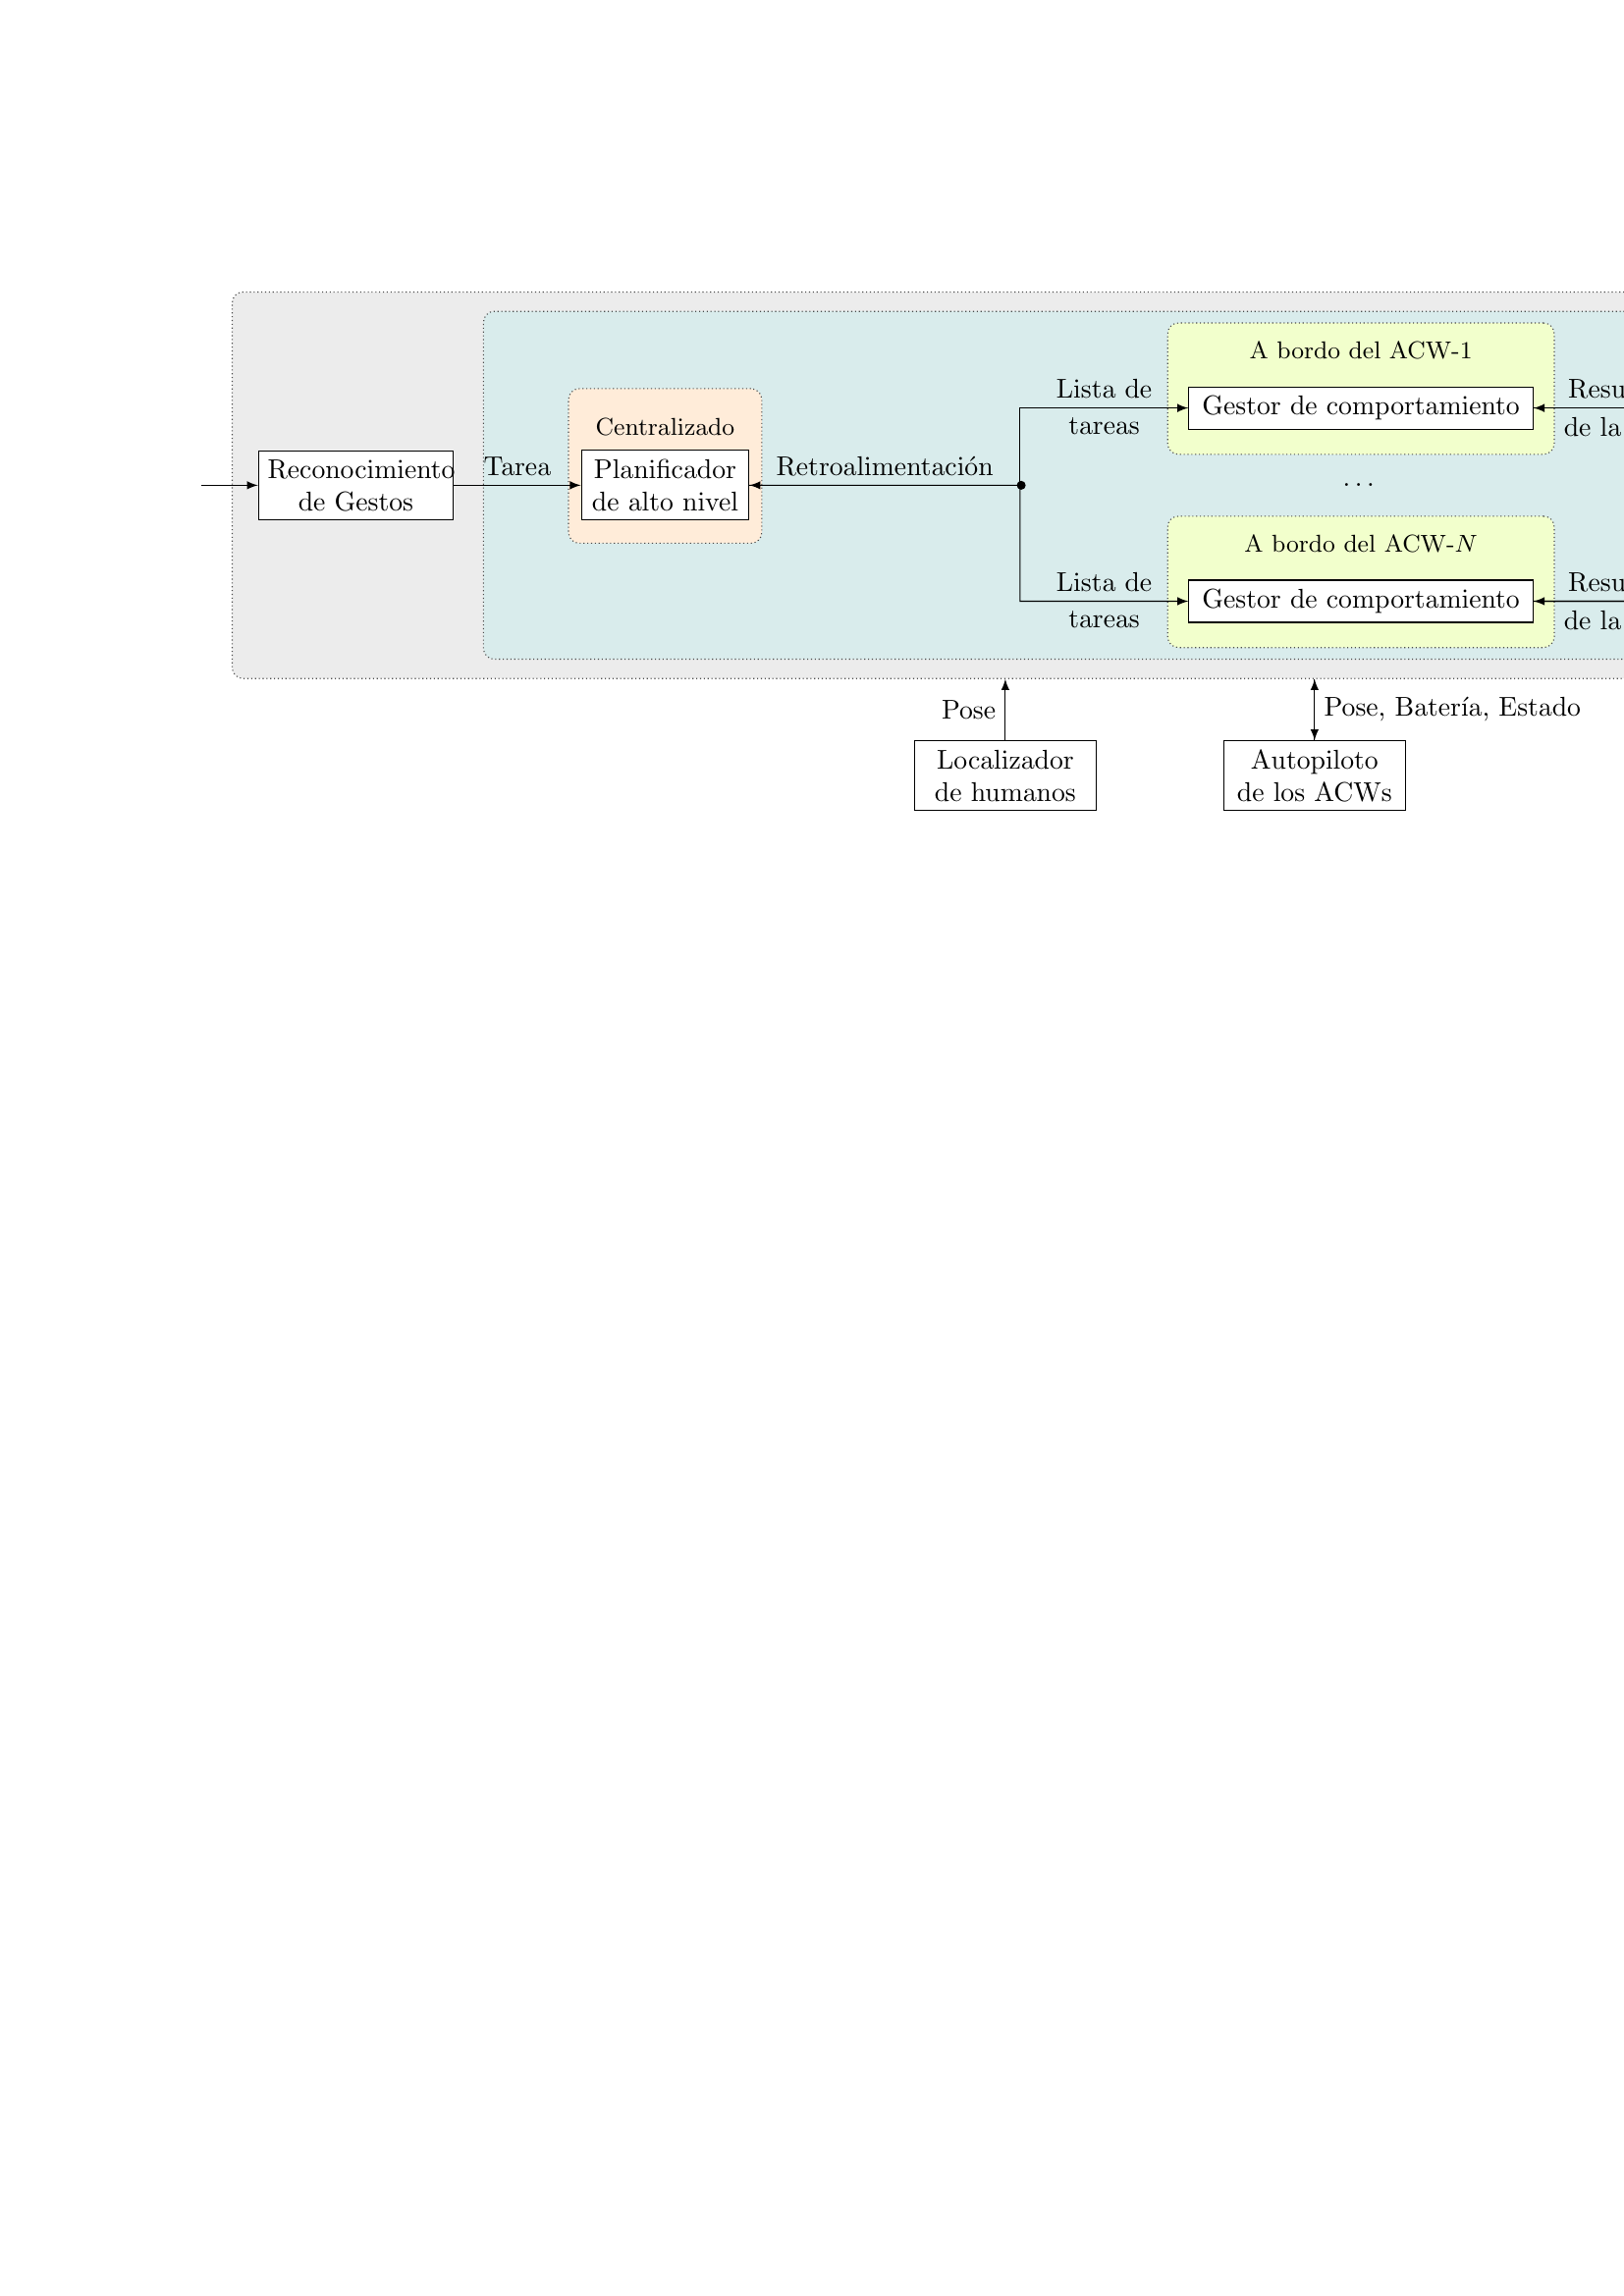
\begin{tikzpicture}
    		% WP7 block
    		\node (WP7-Box) at (10.4,0) [fill=gray!15,rounded corners, draw=black!70, densely dotted, minimum height=5cm, minimum width=24cm]{}; 

			% Task planner box
    		\node (TaskPlannerBox) at ($(WP7-Box)+(0.25,0)$) [fill=teal!15,rounded corners, draw=black!70, densely dotted, minimum height=4.5cm, minimum width=18cm]{};
    		
    		% Gesture Recognition
    		\node (GestureRecognition) at (0,0) [text centered, fill=white, draw, rectangle, minimum width=1.5cm, text width=6.5em]{Reconocimiento\\de Gestos};
    		
    		\draw[-latex] ($(GestureRecognition) - (2,0)$) -- (GestureRecognition);
 
    		% High-Level Planner
    		\node (HighLevelPlannerBox) at ($(GestureRecognition) + (4,0.25)$) [fill=orange!15,rounded corners, draw=black!70, densely dotted, minimum height=2cm, minimum width=2.5cm]{}; 
    		\node (HighLevelPlanner) at ($(HighLevelPlannerBox) + (0,-0.25)$) [text centered, fill=white, draw, rectangle, minimum width=1.5cm, text width=5.5em]{Planificador\\de alto nivel};
    		\node (Centralised) at ($(HighLevelPlanner) + (0,0.75)$) [text centered]{\small Centralizado};
    		
    		\draw[-latex] (GestureRecognition.east) -- node[above]{Tarea} (HighLevelPlanner);
    		
    		%%%%%%%%%%%%%%%%%%%
    		% UAV 1
    		\node (UAV1) at ($(HighLevelPlanner) + (9,1.25)$) [fill=lime!20,rounded corners, draw=black!70, densely dotted, minimum height=1.7cm, minimum width=5cm]{}; 
    		\node (AgentBehaviourManager1) at ($(UAV1) + (0,-0.25)$) [fill=white, draw, rectangle, text centered, text width=12em]{Gestor de comportamiento};
    		\node (UAV1-Text) at ($(AgentBehaviourManager1) + (0,0.75)$) [text centered]{\small A bordo del ACW-$1$};	

    		\draw[fill=black] ($ (HighLevelPlanner.east) + (3.465,0) $) arc(-180:180:0.05);
    		\draw[-latex] (HighLevelPlanner.east) -- ($ (HighLevelPlanner.east) + (3.5,0) $) -- ($ (HighLevelPlanner.east) + (3.5,1) $) -- node[above]{Lista de} node[below]{tareas} (AgentBehaviourManager1.west);
    		\draw[-latex] ($ (HighLevelPlanner.east) + (3.5,0) $) -- node[above]{Retroalimentación} (HighLevelPlanner.east);
    		
    		%%%%%%%%%%%%%%%%%%%
    		
    		% Dots
    		\node (Dots2) at ($(UAV1) + (0,-1.25)$) [text centered]{\dots};
    		
    		%%%%%%%%%%%%%%%%%%%
    		
    		% UAV N
    		\node (UAVN) at ($(HighLevelPlanner) + (9,-1.25)$) [fill=lime!20,rounded corners, draw=black!70, densely dotted, minimum height=1.7cm, minimum width=5cm]{}; 
    		\node (AgentBehaviourManagerN) at ($(UAVN) + (0,-0.25)$) [fill=white, draw, rectangle, text centered, text width=12em]{Gestor de comportamiento};
    		\node (UAVN-Text) at ($(AgentBehaviourManagerN) + (0,0.75)$) [text centered]{\small A bordo del ACW-$N$};	

    		\draw[-latex] (HighLevelPlanner.east) -- ($ (HighLevelPlanner.east) + (3.5,0) $) -- ($ (HighLevelPlanner.east) + (3.5,-1.5) $) -- node[above]{Lista de} node[below]{tareas} (AgentBehaviourManagerN.west);
    		
    		%%%%%%%%%%%%%%%%%%%
    		
    		% Lower-Level Controllers
    		\node (LowerLevelControllers) at ($(HighLevelPlanner) + (17,0)$) [text centered, fill=white, draw, rectangle, minimum width=1.5cm, text width=5.5em]{Controladores\\de nivel inferior};
    		
    		\draw[-latex] (LowerLevelControllers.east) -- ($(LowerLevelControllers) + (1.8,0)$);
    		
    		\draw[fill=black] ($ (LowerLevelControllers.west) + (-2.285,0) $) arc(-180:180:0.05);
    		\draw[-latex] (AgentBehaviourManager1.east) -- ($ (LowerLevelControllers.west) + (-2.25,1) $) -- ($ (LowerLevelControllers.west) + (-2.25,0) $) --  node[above]{Parámetros} node[below]{de la tarea}	(LowerLevelControllers.west);
    		\draw[-latex] (LowerLevelControllers.west) -- ($ (LowerLevelControllers.west) + (-2.25,0) $) -- ($ (LowerLevelControllers.west) + (-2.25,1) $) -- node[above]{Resultado} node[below]{de la tarea}	(AgentBehaviourManager1.east);
    		\draw[-latex] (AgentBehaviourManagerN.east) -- ($ (LowerLevelControllers.west) + (-2.25,-1.5) $) -- ($ (LowerLevelControllers.west) + (-2.25,0) $) -- (LowerLevelControllers.west);
    		\draw[-latex] (LowerLevelControllers.west) -- ($ (LowerLevelControllers.west) + (-2.25,0) $) -- ($ (LowerLevelControllers.west) + (-2.25,-1.5) $) -- node[above]{Resultado} node[below]{de la tarea} (AgentBehaviourManagerN.east);
    		
    		%%%%%%%%%%%%%%%%%%%%%
    		
    		\node (RealUAVs) at ($(WP7-Box.south) + (2,-1.25)$) [text centered, fill=white, draw, rectangle, minimum width=1.5cm, text width=6em]{Autopiloto\\de los ACWs};
    		\node (Humans) at ($(WP7-Box.south) + (-2,-1.25)$) [text centered, fill=white, draw, rectangle, minimum width=1.5cm, text width=6em]{Localizador\\de humanos};
    		
    		\draw[-latex] (RealUAVs.north) -- node[right]{Pose, Batería, Estado} ($(WP7-Box.south) + (2,0)$);
    		\draw[-latex] ($(WP7-Box.south) + (2,0)$) -- (RealUAVs.north);
    		\draw[-latex] (Humans.north) -- node[left]{Pose} ($(WP7-Box.south) + (-2,0)$);
		
	    \end{tikzpicture}}
	\caption{Arquitectura de software: bloques e interfaces. Diagrama de bloques desde la perspectiva del planificador de tareas cognitivas de alto nivel}
	\label{fig:NodeDiagram}
\end{figure}

En el esquema de la arquitectura de software, aunque algunas comunicaciones son bidireccionales, se puede observar que existe un flujo principal de información. Empezando por la información que llega al módulo de \emph{Reconocimiento de Gestos}, ésta se propaga hasta la última capa, donde los \emph{Controladores de nivel inferior} utilizan la información ya procesada para dar órdenes al \glspl{ACW}. La tabla \ref{tab:interfaces} muestra el tipo de datos que cada uno de los módulos de la figura \ref{fig:NodeDiagram} recibe como entrada y el tipo de datos que cada uno de ellos envía como salida. Además, la tabla \ref{tab:shareddata} explica los detalles de los tipos de datos. 

% Description of the data interfaces for each software module
\begin{table}[ht]
    \centering
    \caption{Descripción de las interfaces de datos para cada módulo de software}
    \label{tab:interfaces}
    \small
    \begin{tabular}{|p{0.25\columnwidth}|p{0.25\columnwidth}|p{0.4\columnwidth}|}
      \hline
      \multicolumn{1}{|c}{\textbf{Nombre del módulo}} & \multicolumn{1}{|c|}{\textbf{Dato de entrada}} & \multicolumn{1}{c|}{\textbf{Dato de salida}}\\ \hline \hline
      Reconocimiento de Gestos & Imágenes & \textbf{Tarea, definida por:} ID de la tarea, Tipo de la tarea, Distancia de monitorización, Número de monitorización, Lista de WPs, ID de la herramienta (algunos parámetros de tarea serán ignorados dependiendo del tipo de tarea) \\ \hline
      
     Planificador de alto nivel & Tarea, Retroalimentación (Resultado de la tarea, Batería suficiente, información del árbol de comportamiento (\gls{BT})), Pose del humano, Pose del \glspl{ACW}, Batería y Estado, y Baliza del agente & Lista de tareas añadiendo a cada una sus parámetros extra resultado de la planificación (Formación y/o Lista de IDs de los \glspl{ACW}) y Baliza del planificador\\\hline
      
      Gestor de comportamiento & Lista de tareas, Resultado del nivel inferior, Pose del humano, Pose del \glspl{ACW}, Batería y Estado & Parámetros necesarios para los controladores de bajo nivel (en función del tipo de tarea), Retroalimentación (resultado de la tarea, batería suficiente, información del BT) y Baliza del agente \\ \hline
      
      Controladores de nivel inferior & Parámetros (dependiendo del tipo de la tarea) & Resultado \\ \hline
      
      Localizador de humanos &  & Pose \\ \hline
      
      Autopiloto de los \glspl{ACW} & Órdenes de bajo nivel & Pose, Batería y Estado \\ \hline
      
    \end{tabular}
\end{table}

% Description of data types
\begin{table}[htb]
    \centering
    \caption{Descripción de los tipos de datos}
    \label{tab:shareddata}
    \small
    \begin{tabular}{|p{0.2\columnwidth}|p{0.15\columnwidth}|p{0.55\columnwidth}|}
      \hline
      \multicolumn{1}{|c}{\textbf{Nombre del dato}} & \multicolumn{1}{|c|}{\textbf{Tipo del dato}} & \multicolumn{1}{c|}{\textbf{Comentario}} \\ \hline \hline
      
      ID de la tarea & Cadena & Identificador único de cada tarea \\ \hline
      
      Tipo de tarea & Entero & Indicador del tipo de tarea: m/M, i/I or d/D \\ \hline
      
      ID del humano & Cadena & Identificador único de cada trabajador humano. Se supone que la posición del objetivo humano y otra información necesaria es conocida y accesible a través de su ID. \\ \hline
      
      Distancia de monitorización & Flotante & Distancia desde la que los \glspl{ACW} vigilan al trabajador durante una tarea de monitorización de seguridad  \\ \hline
      
      Número de monitorización & Entero & Número de \glspl{ACW} que se requieren en la formación para una determinada tarea de monitorización de seguridad \\ \hline
      
      Lista de WPs & Lista de tuplas de $3$ flotantes ($x$, $y$, and $z$) & Lista de puntos a inspeccionar \\ \hline
      
      Lista de IDs de \glspl{ACW} & Lists de Cadenas & Lista de los identificadores únicos de los \glspl{ACW} que han sido seleccionados para una tarea que requiere múltiples \glspl{ACW} \\ \hline
      
      Formación & Entero & Indica cuál de los tipos de formaciones predefinidas debe utilizarse para la supervisión (por ejemplo, círculo, triángulo) \\ \hline
      
      ID de herramienta & Cadena & Identificador único de la herramienta a entregar \\ \hline
      
      Pode del \gls{ACW} & geometry\_msgs /PoseStamped & Posición y orientación del \gls{ACW}\\ \hline
      
      Batería del \gls{ACW} & sensors\_msgs /BatteryState & Porcentaje de batería del \gls{ACW} \\ \hline

	    Resultado de la tarea & Cadena, Booleano & El primero es \gls{ID} único de la tarea y el segundo su resultado una vez terminada \\ \hline
      
      Batería suficiente & Booleano & Resultado de calcular si un \gls{ACW} tendrá suficiente batería para su tarea actual \\ \hline

	    Información del \gls{BT} & Lista de Cadenas & Estado de cada nodo de \gls{BT} en su última ejecución (Running, IDLE, SUCCESS or FAILURE) \\ \hline
      
      Baliza del Agente & Cadena, Cadena & El primero es el ID único del \gls{ACW} mientras que el segundo define el tipo de \gls{ACW} (SafetyACW, InspectACW, o PhysicalACW). Se utiliza como latido y para detectar nuevos \glspl{ACW} en el Planificador de alto nivel \\ \hline

	    Baliza del planificador & Tiempo & Mensaje de tipo ROS::Time que contiene el tiempo cuando la baliza fue mandada. Es usado para comprobar el estade de la conexión desde el lado del Agente. \\ \hline
      
      Resultado del nivel inferior & Booleano & Resultado de los controladores de nivel inferior una vez que han terminado después de ser llamados \\ \hline
      
    \end{tabular}
\end{table}

El primer módulo comprueba constantemente las imágenes captadas por el \glspl{UAV} en busca de un gesto que indique una nueva tarea o la modificación de una tarea existente. Cuando esto ocurre, envía asíncronamente una tarea, que será recogida por el planificador centralizado. Como se muestra en la tabla \ref{tab:interfaces}, esta comunicación incluye el \gls{ID} único que diferencia esta tarea de las demás, el tipo de tarea y los parámetros que la definen.

El \emph{Planificador de alto nivel}, cuando recibe esta información, procede a reevaluar el plan óptimo teniendo en cuenta la tarea recibida, la información que recibe de los \emph{Autopilotos de los \glspl{ACW}}, y la posición de los operarios, que es publicada periódicamente por el \emph{Localizador de humanos}. Estos datos constituyen la entrada para el \emph{Planificador de alto nivel}, junto con la información procedente de cada \emph{Gestor de comportamiento} de los agentes. Su salida es una lista de tareas para cada \gls{ACW}.

A bordo de cada \gls{ACW} hay un \emph{Gestor de comportamiento} de agente. Este módulo se encarga de recoger la correspondiente lista de tareas proporcionada por el planificador centralizado. Con esta entrada y la información procedente del \emph{Localizador de humanos} y del \emph{Autopiloto del \gls{ACW}}, este módulo se encarga de llamar a los \emph{Contoladores de nivel inferior} para llevar a cabo la ejecución del plan asignado. La información emitida por el \emph{Autopiloto del \gls{ACW}} se utiliza también para comprobar que todo funciona correctamente y para ejecutar los protocolos de seguridad en caso de que sean necesarios. Si esto ocurriera, se emitiría la correspondiente comunicación de vuelta al \emph{Planificador de alto nivel} para calcular un nuevo plan. Estos módulos también reciben el resultado de los \emph{Controladores de nivel inferior} después de llamar a cada uno de ellos, y lo publican de vuelta al \emph{Planificador de alto nivel} como retroalimentación.

Además de estas comunicaciones, los módulos \emph{Planificador de alto nivel} y \emph{Gestor de comportamiento} de agente intercambian periódicamente balizas que sirven para detectar tanto la conexión de un nuevo \gls{ACW} como su desconexión en caso de fallo. Además, existe una comunicación asíncrona que se emite a todos los componentes indicando el final de la misión cuando ésta se produce.

Por último, cabe mencionar que el módulo \emph{Reconocimiento de gestos} no tiene una comunicación destinada a modificar los parámetros de una tarea ya contemplada dentro del \emph{Planificador de alto nivel}. Sin embargo, esto es posible porque las tareas tienen un identificador único. Una vez que una tarea ha sido entregada al \emph{Planificador de alto nivel}, para cambiar alguno de sus parámetros, el módulo \emph{Reconocimiento de gestos} sólo tiene que enviar la tarea de nuevo, manteniendo el mismo \gls{ID} de la tarea y actualizando sólo los parámetros deseados. Así, dentro de la función que se ejecuta cuando se comunica una nueva tarea, se llama a otra función para actualizar los parámetros de las tareas ya registradas.

\section{Módulo centalizado: Planificador de alto nivel}
\label{sec:Centralised module:TaskPlanner}
Como se ha mencionado anteriormente, el \emph{Planificador de alto nivel} es un módulo centralizado que se ejecuta en una estación terrestre y constituye el principal módulo cognitivo de la arquitectura de software. Su objetivo es planificar la misión de forma óptima, es decir distribuir las tareas pendientes entre los \glspl{ACW} disponibles especificando el orden en el que se van a ejecutar, teniendo en cuenta el tiempo que se tarda en completar cada una, el tipo de cada \glspl{UAV}, la distancia que tendrá que recorrer cada uno, la batería que tienen disponible, la tarea que estaba ejecutando cada uno, la prioridad de cada tarea, la batería consumida por cada tarea, las recargas que serán necesarias, y cuándo es mejor realizar esas recargas.

El pseudocódigo general de este componente, desde el lanzamiento hasta la terminación, está representado en el código \ref{ps:GeneralPlanner}.

\begin{lstlisting}[caption={General operation of \emph{High-Level Planner}'s code}, breaklines=true, label=ps:GeneralPlanner]
  1. Leer de un ros::param la dirección del archivo de configuración.
	2. Leer del archivo de configuración toda la información necesaria.
	3. Configurar las comunicaciones ROS (Publishers, Subscribers y ActionServers).
	4. Configurar la frecuencia de bucle.
	5. Bucle "while" principal". Mientras que ros::ok() y no misión terminada hacer:
		5.1. Comprobar el tiempo transcurrido de las balizas de los Agentes.
		5.2. Publicar una nueva baliza del Planificador.
		5.3. Comprobar si hay comunicaciones entrantes pendientes (ros::spinOnce).
		5.4. Dormir el tiempo restante para enviar la siguiente baliza.
	6. 6. Esperar a que todos los UAVs terminen y se desconecten. Mientras que haya algún agente conectado hacer:
		6.1. Comprobar el tiempo transcurrido de las balizas de los agentes.
		6.2. Comprobar si hay comunicaciones entrantes pendientes (ros::spinOnce).
		6.3. Dormir un rato.
\end{lstlisting}

Dado que el entorno en el que operan los \glspl{UAV} es dinámico, este módulo se ha programado de forma que pueda reaccionar ante los imprevistos y recalcular el plan óptimo. Como se puede deducir del código \ref{ps:GeneralPlanner}, todo funciona a través de funciones de respuesta. Cada vez que llega una comunicación desde otro nodo de \acrshort{ROS}, se activa una respuesta en este nodo. En ella se analiza la información contenida en el mensaje y se decide si es necesaria una replanificación o no. Las situaciones en las que se ha considerado necesaria una replanificación se enumeran en la sección \ref{sec:TaskReplanningSituations}. Las comunicaciones resumidas en las tablas \ref{tab:interfaces} y \ref{tab:shareddata} y en la figura \ref{fig:NodeDiagram} son suficientes para detectar estos imprevistos y poder responder a ellos de la mejor manera posible.

\begin{lstlisting}[caption={Task callback pseudocode}, breaklines=true, label=ps:IncomingTask]
	1. If the task already exists:
		1.1. If the new task's type is the same as old one's type:
			1.1.1. Update parameters, perform a task planning and return.
		1.2. Else: Warn operators that a pending task is going to be deleted and delete old task.
	2. Read the type of task and the parameters that apply to it.
	3. Add the new task to the pending task list.
	4. Perform a task planning.
\end{lstlisting}

There is a callback that is executed when the node \emph{Gesture Recognition} sends a task, which in case the given task is correct, always ends up calling the function in charge of calculating the optimal plan (see Code \ref{ps:IncomingTask}); the mission over callback, whose only action is to change the value of a variable so that the node exits the main while loop; and finally the agent's beacon callback, which is executed every time a \gls{UAV} beacon is received and whose pseudocode is in Code \ref{ps:AgentBeaconCallback}.

\begin{lstlisting}[caption={Agent's beacon callback}, breaklines=true, label=ps:AgentBeaconCallback]
	1. Read the information contained in the beacon.
	2. If it is a connection of a new UAV:
		2.1. Register it in the database.
		2.2. Perform a task planning.
	3. Else, if it is the heartbeat of an already known UAV:
		3.1. Reset the timeout timer.
\end{lstlisting}

The action carried out by the agent's beacon callback varies depending on whether it is the beacon of a new \gls{UAV} or the heartbeat of a known \gls{UAV}. For each agent there will be an object in the database that will contain another series of callbacks that will be in charge of receiving the messages coming from the \glspl{ACW} and respond accordingly.

\begin{lstlisting}[caption={Callback that runs when an \emph{Agent Behaviour Manager} sends battery feedback}, breaklines=true, label=ps:batteryEnoughCB]
	1. Update the value of the internal flag associated with the battery.
	2. Perform a task planning.
\end{lstlisting}

The \emph{Agent Behaviour Manager} block only sends communications messages indicating the battery status when it is due to an unplanned event. This event can be either an early battery depletion or a faster than expected recharge. In both cases, the callback function, whose pseudocode is Code \ref{ps:batteryEnoughCB}, updates the value of an internal variable used during planning, and recalculates the optimal plan.

The other possible communication coming from a node of type \emph{Agent Behaviour Manager} with the ability to trigger a reaction in the planner is due to the termination of a task. When a task finishes successfully, it is simply removed from the list of pending tasks. In this case, the emph{Agent Behaviour Manager} block also removes the task from its queue, which is the only case where it does so. In addition, this moment is used to re-evaluate the optimal plan. It is expected that the mission is still within the optimal plan, so in that case the planning result should be the same as the plan that was already being executed. If, instead, conditions have changed since the last planning and there exists a better plan now, it is at this point that the plan is updated. If the task ends with a failure, the callback action will depend on the causes of the failure (note that the interruption of a task will result in a failure). If the interruption is due to the \gls{UAV} battery, it may be planned, in which case no action is required, or it may be unexpected, in which case the corresponding actions are taken by the battery callback. Once it has been verified that the task has not finished due to the battery, a check is made to see if the task was at the beginning of the queue. If so, a failure has indeed occurred, so the operators are warned, the task is removed from the list, and a replanning is executed. Otherwise the task in question would have been moved from the top of the queue due to a change of plans and therefore no action would have to be taken either. The pseudocode corresponding to what has just been explained is in Code \ref{ps:taskResultCB}.

\begin{lstlisting}[caption={Callback that runs when an \emph{Agent Behaviour Manager} sends a task result}, breaklines=true, label=ps:taskResultCB]
	1. Read the information contained in the task result.
	2. If the task result is SUCCESS:
		2.1. Delete it from the pending tasks list.
		2.2. Perform a task planning.
	3. Else, if the task result is FAILURE:
		3.1. If the task has been halted because of not having battery enough:
			3.1.1. Return.
		3.2. Else, if the task is on the front of that ACW's task queue:
			3.2.1. Notify operators that a task has failed and is going to be deleted.
			3.2.2. Delete task from the pending tasks list.
			3.2.3. Perform a task planning.
		3.3. Else:
			3.3.1. Return.
\end{lstlisting}

The other two communications received by the \emph{High-Level Planner} from the \glspl{ACW} are sensor readings corresponding to the \glspl{UAV}' position and battery percentage. In both cases the only action of the corresponding callback is to update the information with the new values.

The last function that remains to be explained of those that can potentially request a replanning of the mission is the one in charge of checking the timeout of the agents' beacons. As shown in  Code \ref{ps:GeneralPlanner}, this function is not a callback like the previous ones, instead it is executed periodically in the main while loop. Its operation is shown in Code \ref{ps:checkBeaconsTimeout}. Basically, for each agent connected, it checks that the timeout amount of time has not elapsed since its last beacon was received. If a timeout has occurred, that \gls{ACW} is considered disconnected and is removed from the centralised node data. If, after checking all agents, the number of connected \glspl{UAV} has decreased, i.e. if any of the previously connected \glspl{UAV} has disconnected, a mission replanning is executed.

% Pseudocódigo de checkBeaconsTimeout
\begin{lstlisting}[caption={Beacons' timeout check function}, breaklines=true, label=ps:checkBeaconsTimeout]
	1. For each agent connected:
		1.1. If the elapsed time since the last beacon is greater than the timeout time:
			1.1.1. Add that agent's ID to the list of disconnected agents.
	2. While the list of disconnected agents is not empty:
		2.1. Take first ID from the list.
		2.2. Erase from the block's data all information related to that ID.
	3. If any agent has been disconnected:
		3.1. Perform a task planning.
\end{lstlisting}

%% Explicar como se realiza la planificación y poner psudocódigo de cómo se lleva a cabo. Explicar también como se calcula el coste.
The pseudocode that is executed when one of these functions deems it necessary to perform a new task planning is summarised in Code \ref{ps:performTaskAllocation}. It is important to remember that some tasks have a higher priority than others, and this depends only on the type of task. To simplify the process, it has been decided to allocate the tasks in order of arrival, assuming that between two tasks of the same type, the one that arrived first will have priority. When a new task is received, it is stored both in a \emph{std::map} that contains all the pending tasks to facilitate the access to the information, and in a \emph{std::vector} with task types, where the order of arrival is maintained. What this simplification allows is to assign tasks one at a time. By having a prioritised list of tasks and assuming that no task can be assigned before a task with a higher priority, the mission planning problem is reduced to calculating the cost of each task individually for each \gls{UAV} with the ability to execute it and assign it to the one with the lowest cost. For monitoring-type tasks, the selection of the required number of agents is strictly cost-based. The \emph{N} agents that cost the least to execute the task are selected. The same is a little more complex for the tasks of type inspect, where the number of agents to select is a parameter to be defined by the planner itself. This value is first set according to the number of points to be inspected. Up to three points, a single \gls{ACW} is selected; up to six points, two are selected; and from seven points onwards, three agents are selected, this being the maximum number imposed by the low-level controller. Moreover, as the low-level controller in charge of this task works, all the \glspl{ACW} selected for this task are required to start executing it simultaneously, so a second approximation of this number is made according to the number of idle \glspl{UAV}. Thus, if they are assigned this as the first task, they will start executing it simultaneously. Academically, this simplification seems to deviate from the optimal solution, but it should be recalled that this work is part of a software architecture that will operate in real situations. In such situations, it is not expected that there will be a large number of \glspl{UAV} connected simultaneously, nor a long list of pending tasks. In such simplified scenarios, this assumption makes sense without deviating too much from the optimal solution. Finally, the number of agents to be selected will be the smaller of the two above, being equal to one when there is no \gls{UAV} idle and zero in case there is no \gls{ACW} with enough battery. In the latter case, the task would be assigned after recharging. Once the number of agents to be selected has been defined, the agents that have the least cost to execute the task are selected from among those that meet the conditions described. Having selected the \gls{ACW} that will carry out the task, all that remains is to distribute among them the \glspl{WP} to be inspected. Although the algorithm in charge of performing the optimal distribution is in the low-level controller of this task, as the rest of the modules that make up the software architecture are not yet available, it has been necessary to program a distribution algorithm in order to be able to carry out the experiments. More details on this will be given in Section \ref{sec:faking}.

% Explicar como se calcula el coste.
The cost for each \gls{UAV} is calculated as the weighted sum of three different types of costs. A first cost assesses the type of \gls{ACW} and penalises the assignment of tasks to those \glspl{UAV} designed for another type. It penalises especially the assignment of lower priority tasks to agents designed to perform higher priority tasks. The second cost evaluates the total distance the \gls{UAV} will have to travel from where it is at the beginning of the task to where it should be by the end of the task. This cost is an approximation of the expected battery consumption, although it does not take into account intermediate travel and hoovering times during the mission. The last cost penalises the interruption of the task that was being executed according to the previous plan and rewards the assignment of the same task. This cost is intended to ensure that a task is preferentially assigned to an idle \gls{UAV}, to an \gls{UAV} that is executing a lower priority task, or even to an \gls{UAV} of a different type, rather than interrupting a task unnecessarily just because that \gls{ACW} has to travel a shorter distance, for example.

\begin{lstlisting}[caption={Task planning function's pseudocode}, breaklines=true, label=ps:performTaskAllocation]
	1. If there is any agent connected:
		1.1. For each agent connected:
			1.1.1. Make a copy of the current task queue.
			1.1.2. Empty the task queue.
		1.2. For each Tool Delivery task:
			1.2.1. Compute the cost of the task for each PhysicalACW that has enough battery.
			1.2.2. Assign the task to the agent for whom the task costs the least (from those who has enough battery).
			1.2.3. Add the task to that agent's task queue.
		1.3. For each Inspection task:
			1.3.1. Extract from the task parameters the list of WP to inspect.
			1.3.2. For each ACW (any type) that has enough battery:
				1.3.2.1. Compute the cost of the task for that ACW. 
				1.3.2.2. Check if that ACW is still idle.
			1.3.3. Calculate the number of agents to select for the task based on the number of WP and the number of idle agents.
			1.3.4. If no agent has enough battery, continue.
			1.3.5. Else, if the number of agents to select is equal to zero, assign the task to the agent that costs the least.
			1.3.6. Else, select the calculated number of agents for whom the task costs the least.
			1.3.7. Divide the WP to inspect among the selected agents.
			1.3.8. For each selected agent:
				1.3.8.1. Set the remaining task parameters (List of selected ACWs' IDs and divided WP list).
				1.3.8.2. Add the task to the agent's task queue.
		1.4. For each Monitoring task:
			1.4.1. Compute the cost of the task for each ACW (any type) that has enough battery.
			1.4.2. If the required number of ACWs for the task is zero:
				1.4.2.1. Warn operators that this parameter can not be zero.
				1.4.2.2. Delete task from pending tasks.
			1.4.3. Else, select the requested number of agents for whom the task costs the least.
			1.4.4. Set the remaining task parameter (List of selected ACWs' IDs)
			1.4.4. Add the task to each selected agent's task queue.
		1.5. For each ACW connected, send the new task queue to its Agent Behaviour Manager.
	2. Else:
		2.1. Warn operators that no agent is connected.
\end{lstlisting}

Once the calculation of the mission plan has been completed, the new task queues are sent to the corresponding distributed modules. Each \emph{Agent Behaviour Manager} will react to this communication and will take care of executing the newly assigned plan. In the meantime, the \emph{High-Level Planner} block returns to the main while loop to continue waiting until an event that triggers a replanning occurs again.

\section{Distributed module: Agent Behaviour Manager}
\label{sec:Distributed module: behaviour manager}
%% Explicar qué es una drone behavior manager y cual es su función.
This component is in charge of executing the plan assigned by the \emph{High-Level Planner}, checking the security of the \glspl{UAV} at all times, detecting unforeseen events and communicating them to the centralised node so that it can make a change of plans if needed. The \emph{Agent Behaviour Manager} will communicate with the low-level controllers, handing over control when necessary to complete the assigned plan.

%% Estructura general del nodo (pseudocodigo). Explicar que se ha hecho con árboles de comportamiento en paralelo a algunos procesos de ros
The general structure of this module is quite similar to that of the central module. The pseudocode is summarised in Code \ref{ps:GeneralAgent}. Upon initialisation, the \emph{Agent Behaviour Manager} prepares the necessary information to start its operation, configures the necessary communications, declares and initialises the behaviour tree and, once the \gls{UAV} has finished initialising, starts sending beacons to the central node to notify that it is joining the mission. Once the code finishes initialising and reaches the main while loop, the activity of the \emph{Agent Behaviour Manager} concentrates on the execution of callbacks in response to incoming messages, as in the \emph{High-Level Planner}, and on the execution of the behaviour tree, which directs and supervises the \gls{UAV} movement.

\begin{lstlisting}[caption={General operation of \emph{Agent Behaviour Manager}}, breaklines=true, label=ps:GeneralAgent]
	1. Read from a ros::param the beacon's content (ACW's ID and type).
	2. Read from a ros::param the address of the configuration file.
	3. Read from the configuration file all necessary information.
	4. Configure ROS communications (Publishers, Subscribers and ActionServers).
	5. Set the loop rate.
	6. Declare the behaviour tree.
	7. Initialise each BT node.
	8. Start BT loggers to facilitate debugging and monitoring of the node's performance.
	9. Wait until the ACW fully initialises.
	10. Main "while" loop. While ros::ok() and BT status is running:
		10.1. If a timeout of Planner's beacons has not ocurred:
			10.1.1. Publish a new Agent beacon.
		10.2. Check if battery is enough for the current task.
		10.3. Check for pending incoming communications (ros::spinOnce).
		10.4. Sleep the remaining time to send the next beacon.
\end{lstlisting}

%% Explicar lo que es un árbol de comportamiento y compararlo con una máquina de estados.
The \glspl{BT} are who governs the \glspl{ACW} to perform each of the assigned tasks. Each \gls{BT} monitors its \gls{ACW}'s battery and task status and reacts to any possible failure or unexpected event, requesting a new re-planning to the \emph{High-Level Planner} in case of need. A \gls{BT} can be defined as an improved \gls{FSM}. They are a more advanced mechanism to implement behaviours, especially because of their advantages in terms of scalability, modularity, readability and reusability, facilitating the creation of more complex behaviours with less effort.

%% Diseño del árbol de comportamiento.
Despite this, the process of designing a state machine is quite different from the process of designing a behaviour tree. Designing behaviour trees without ever having done it before is not a trivial task. Moreover, there will be more than one valid implementation to achieve the same behaviour, which makes it more complicated to design this type of solution when you do not still have enough intuition to know which one is better. Taking advantage of the fact that the use of \glspl{BT} is widespread in the videogame industry, information about them was gathered and studied to try to develop enough knowledge and intuition to design from scratch a \gls{BT} that meets the needs of the mission. For that, previous examples found in \cite{BT-CPP-doc, colledanchise2018behavior, BT-AI} were very useful.

Before proceeding with the explanation of the designed \gls{BT}, the types of nodes that can be found in the selected C++ library (see Figure~\ref{fig:BTnodes}) and the functioning of each of them will be briefly discussed.

%% Tipos de nodos de BT
\begin{figure}[htbp]
    \centering
    \subfloat[]{%Fallback
		\label{subfig:Fallback}
        \begin{tikzpicture}
			\node (MainTree) at (0,0) [text centered, fill=white, draw, rectangle, minimum width=0.5cm, text width=0.5em]{\textbf{?}};
		\end{tikzpicture}}
    \hfill
    \subfloat[]{%Sequence
		\label{subfig:Sequence}
        \begin{tikzpicture}
			\node (MainTree) at (0,0) [text centered, fill=white, draw, rectangle, minimum width=1.5cm, text width=1.5em]{$\longrightarrow$};
		\end{tikzpicture}}
	\hfill
    \subfloat[]{%Reactive
		\label{subfig:Reactive}
        \begin{tikzpicture}
			\node (MainTree) at (0,0) [text centered, fill=magenta!5, draw=magenta, rectangle, minimum width=2cm, minimum height=0.75cm, text width=2em]{};
		\end{tikzpicture}}
    \hfill
    \subfloat[]{%Common
		\label{subfig:Common}
        \begin{tikzpicture}
			\node (MainTree) at (0,0) [text centered, fill=white, draw, rectangle, minimum width=2cm, minimum height=0.75cm, text width=2em]{};
		\end{tikzpicture}}
    \hfill
    \subfloat[]{%Decorator
		\label{subfig:Decorator}
        \begin{tikzpicture}
			\node (MainTree) at (0,0) [text centered, fill=orange!5, draw=orange, rectangle, minimum width=2cm, minimum height=0.75cm, text width=2em]{};
		\end{tikzpicture}}
    \hfill
    \subfloat[]{%Action
		\label{subfig:Action}
		\begin{tikzpicture}
			\node (MainTree) at (0,0) [text centered, fill=blue!5, draw=blue, rectangle, minimum width=2cm, minimum height=0.75cm, text width=2em]{};
		\end{tikzpicture}}
		\hfill
    \subfloat[]{%Condition
		\label{subfig:Condition}
        \begin{tikzpicture}
			\node (MainTree) at (0,0) [text centered, fill=blue!5, draw=blue, ellipse, minimum width=2cm, minimum height=0.75cm, text width=2em]{};
		\end{tikzpicture}}
    \caption{Different types of nodes that can be present in an \gls{BT}}
    \label{fig:BTnodes}
\end{figure}

 Behaviour Trees are made up of \emph{Control} nodes, \emph{Decorator} nodes, and \emph{Leaf} nodes. \emph{Control} nodes could be either \emph{Fallback} nodes, represented with a question mark (see subfigure \ref{subfig:Fallback}), which try success calling one by one each of their children; or \emph{Sequence} nodes, represented with an arrow (see subfigure \ref{subfig:Sequence}), which call their children in order if the previous one has succeeded. On the one hand, \emph{Fallback} nodes return \emph{SUCCESS} if one of its children does it, \emph{FAILURE} if none of them success, and \emph{RUNNING} if one of its children returns \emph{RUNNING}. On the other hand, \emph{Sequence} nodes return \emph{SUCCESS} when all children have been called in order and have returned \emph{SUCCESS}. If any of them returns \emph{FAILURE}, the sequence is broken and the \emph{Sequence} node returns \emph{FAILURE} too. When a child returns \emph{RUNNING}, the \emph{Sequence} node does it too. \emph{Control} nodes are represented in a black rectangular box when they are the standard ones (see subfigure \ref{subfig:Common}), but they could also be \emph{Reactive} control nodes, represented by a magenta box (see subfigure \ref{subfig:Reactive}), which means that its already called children will be called again in the next iteration. This is very useful for generating behaviours where an action is constantly reattempted, or where it is necessary to check that the required conditions are still met. A \emph{Child} node could be another \emph{Control} node, a \emph{Decorator} node, a \emph{Leaf} node or a whole sub-tree. A \emph{Decorator} node, represented in an orange box (see subfigure \ref{subfig:Decorator}), can only have one child (of any type) and its function is programmable (e.g., modifying its child result or retrying calling its child a number of times). \emph{Leaf} nodes, represented in blue, could be \emph{Condition} nodes, represented in a blue elliptical shaped box (see subfigure \ref{subfig:Condition}), that check a condition and return either \emph{SUCCESS} or \emph{FAILURE}; or \emph{Action} nodes, represented in a blue rectangular box (see subfigure \ref{subfig:Action}), that execute code that takes longer and therefore these nodes could also return \emph{RUNNING}.

\subsection{Main tree}
\label{sec:MainTree}
In general, the design of both the behaviour tree and the \emph{Agent Behaviour Manager} has been made with the aim of concentrating as less intelligence as possible, to ensure the success of the mission and the safety of the \glspl{UAV} and the workers. That is why the only task of the callback functions that are executed when different messages come in is to update the value of the corresponding internal variables. 

However, not all intelligence and decision-making can be placed in the ground station node. There has to be some decision-making capability on board \glspl{UAV} in case the connection to the central node is lost. That is why there is a predefined protocol to act when this happens or when the battery runs out of power earlier than expected. These two factors are periodically checked in the main while loop (see Code \ref{ps:GeneralAgent}). In the case of the battery, if the function in charge determines that there is not enough battery to complete the current task, what happens is that the task queue is emptied and the value of the internal flag associated with the battery is updated. In addition, the event is communicated to the task planner in case the connection is still alive to generate a new plan. Similarly, if a connection loss is detected, the task queue is emptied and the corresponding flag is updated. In this case the \emph{High-Level Planner} node will execute a replanning when it also detects the connection loss.

The behaviour tree is designed in such a way that, when the task queue is emptied and the respective flags are updated, the corresponding \gls{UAV} goes to the battery charging station, which is the established emergency protocol. In order to justify this decision, each of the cases will be analysed separately below.

In case the connection between the two nodes is still active but there is not enough battery, the aim of the contingency plan is to eliminate risks to the \gls{UAV} while the \emph{High-Level Planner} generates new instructions. In addition, the new plan is likely to involve recharging the battery as a first step. Besides, there is a possibility that the connection may be lost at this point.

The danger of connection loss is that the \emph{High-Level Planner} will replan the mission without the disconnected \gls{ACW}, so that the tasks previously assigned to it will now be executed by others. If in this scenario the disconnected \gls{ACW} continues with the last assigned plan, collisions could occur. The emergency protocol ensures that the disconnected \gls{UAV} does not interfere with the new plans. In addition, the time until the connection is re-established is used by recharging the battery, which is positive for the mission.

%%%%%%%%%%%%%%%%%%% El Agent Behavior Manager no elimina nunca una tarea de la cola en la revión actual. ¿Eso lo omito o debería explicarlo?

\glspl{BT} operate recursively. All nodes, regardless of their type, have a function that executes their content, the \emph{tick} function. When the root node is \emph{ticked} from the main while loop, it propagates the \emph{tick} among its children following the operation rules described in Section \ref{sec:Distributed module: behaviour manager} until eventually a \emph{leaf} node returns one of three possible responses (\emph{SUCCESS}, \emph{RUNNING} or \emph{FAILURE}), which will be propagated back, to obtain a final result that the root node will return. 

Typically, a \gls{BT} is executed to achieve a goal, and therefore the executor keeps on doing \emph{tick} to the tree root until the response is either \emph{SUCCESS} or \emph{FAILURE}. As the function of this \gls{BT} is to control during the whole mission the movement of a \gls{UAV}, it is of interest that the result of the root is \emph{RUNNING} until the mission ends. This is why a \emph{Decorator} node that always returns \emph{RUNNING} regardless of the result of its child node has been defined. The \gls{BT} implemented as a solution for the described problem is further divided into several \glspl{BT}, taking advantage of the modularity offered by this approach. The main tree is represented in Figure \ref{fig:MainTree}, being the node named as \emph{Main Tree} the root of the complete tree.

\begin{figure}[ht]
	\begin{center}
		\scalebox{0.9}{
			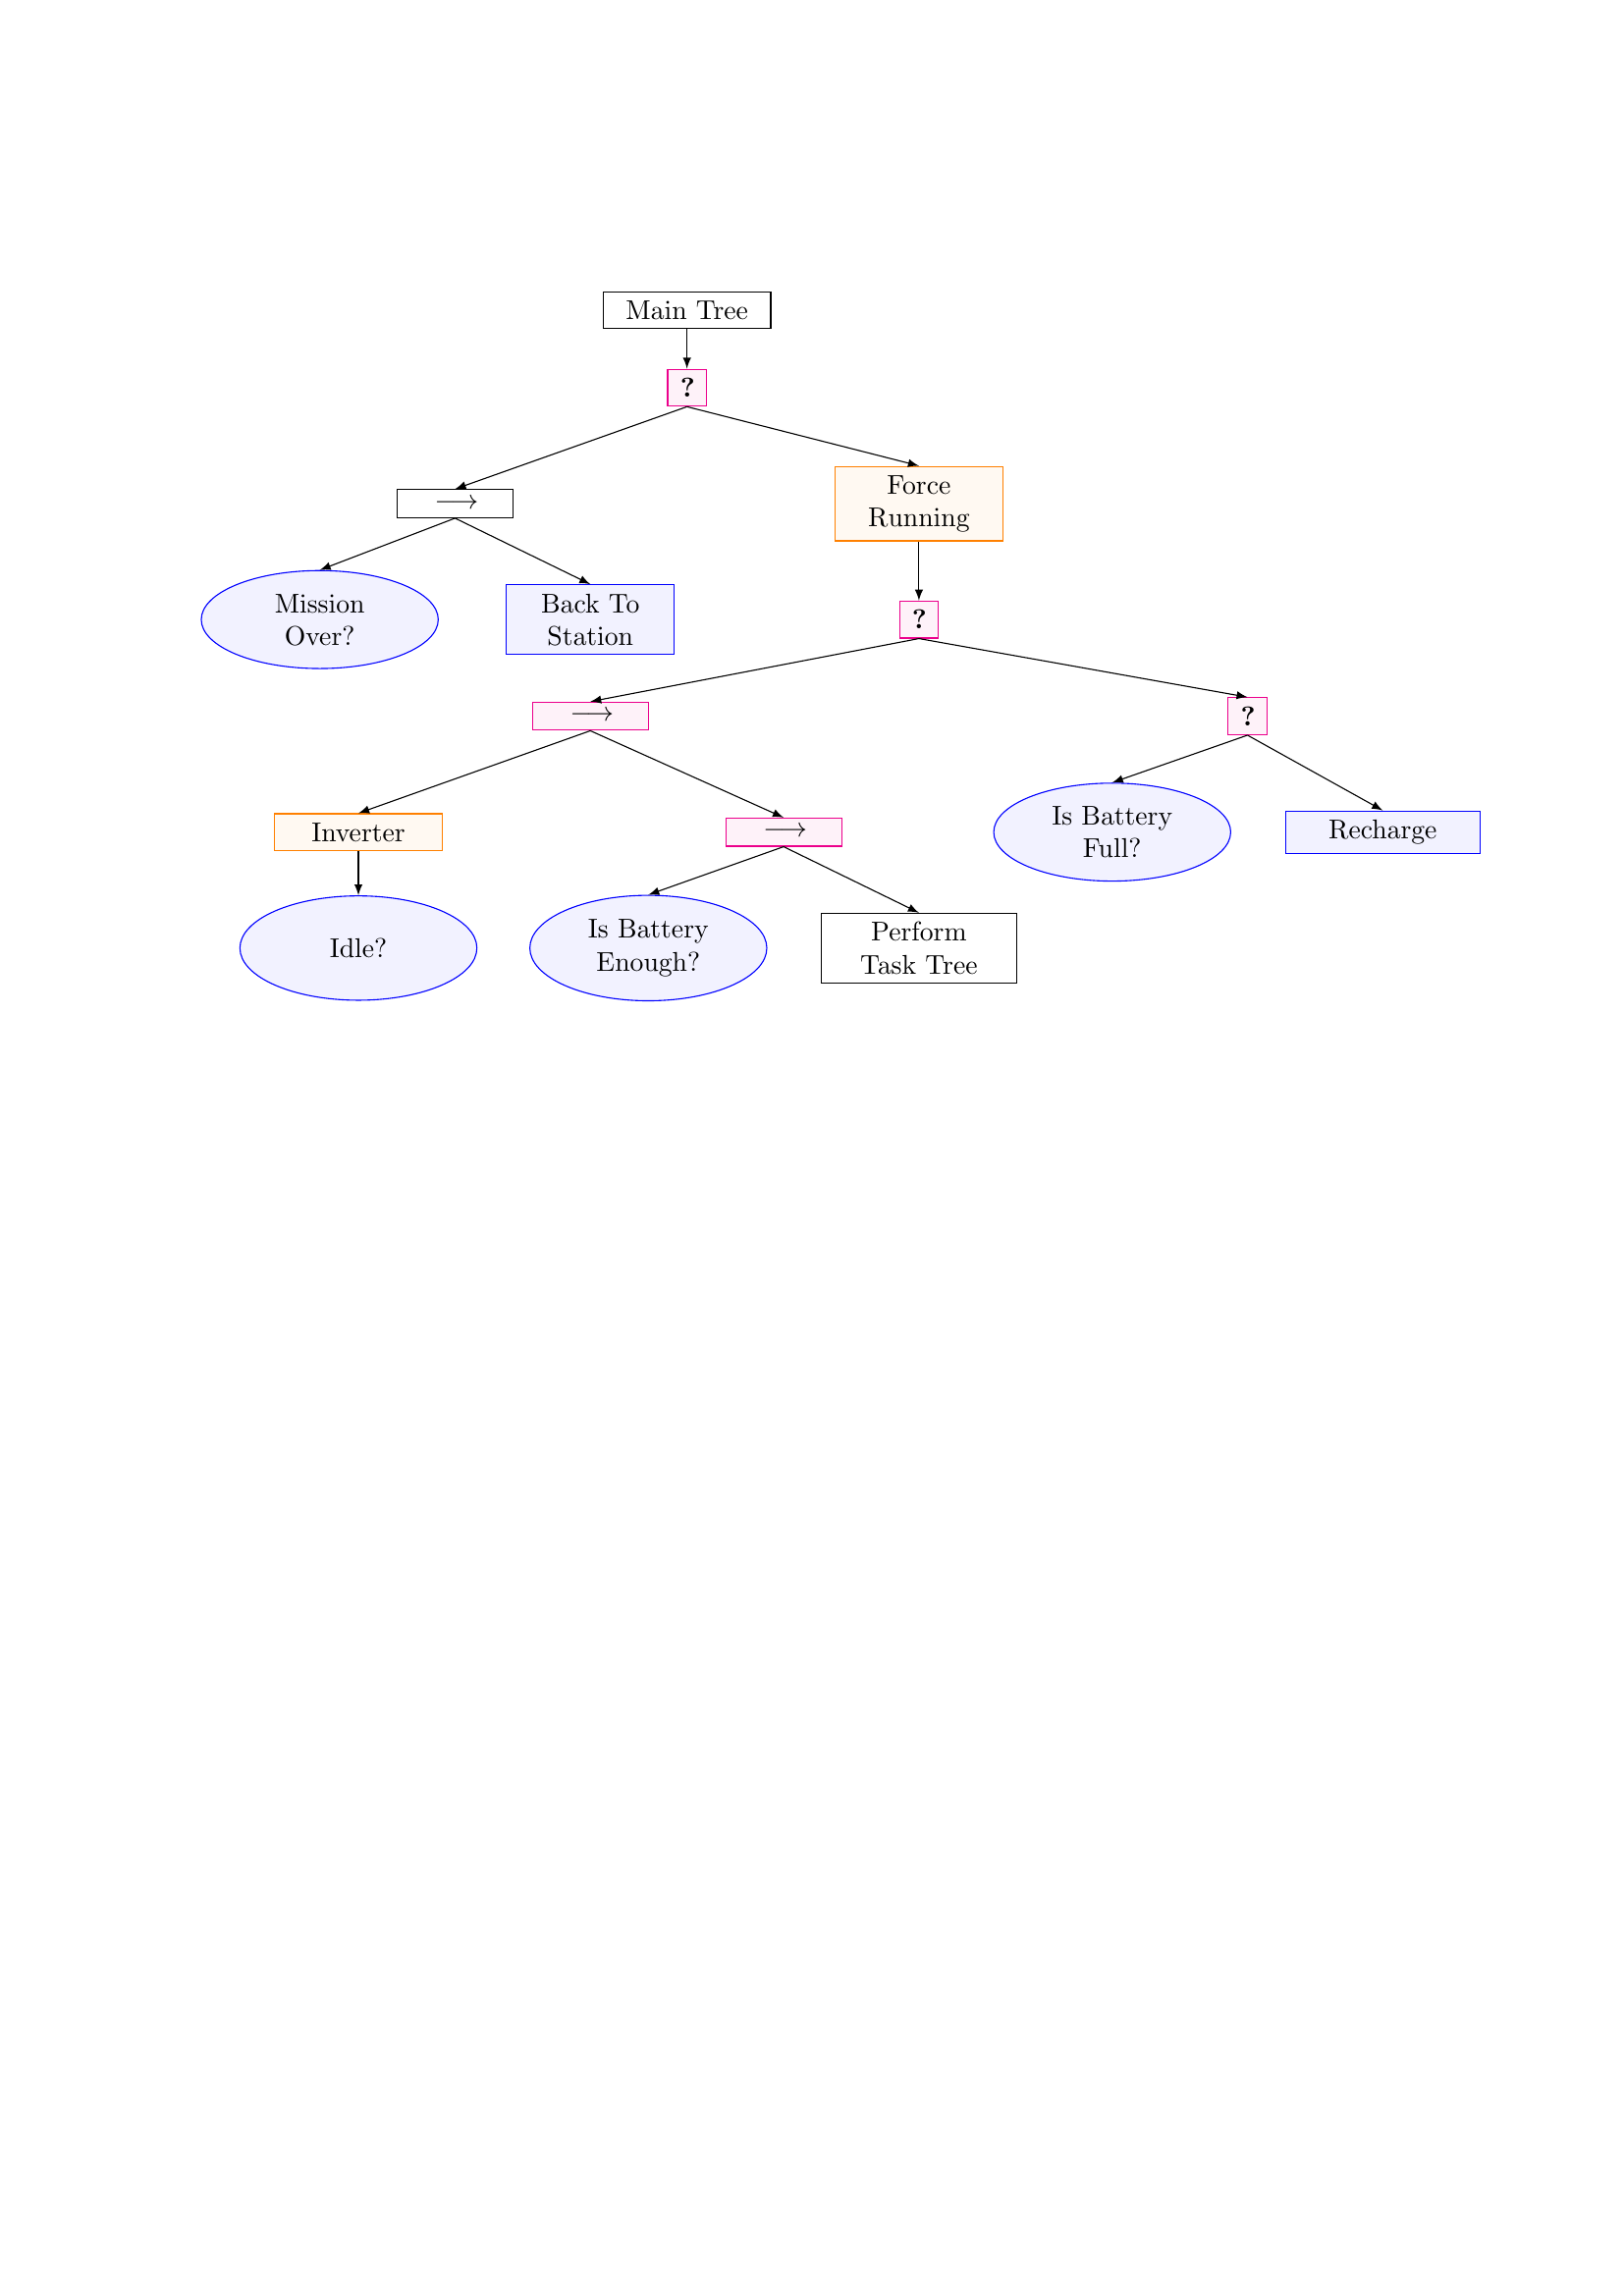
\begin{tikzpicture}
        		\node (MainTree) at (0,0) [text centered, fill=white, draw, rectangle, minimum width=1.5cm, text width=5.5em]{Main Tree};

        		\node (RootFallback) at ($(MainTree) + (0,-1)$) [text centered, fill=magenta!5, draw=magenta, rectangle, minimum width=0.5cm, text width=0.5em]{\textbf{?}};
        		\draw[-latex] (MainTree.south) -- (RootFallback.north);

        		\node (MissionOverSequence) at ($(RootFallback) + (-3,-1.5)$) [text centered, fill=white, draw, rectangle, minimum width=1.5cm, text width=1.5em]{$\longrightarrow$};
        		\draw[-latex] (RootFallback.south) -- (MissionOverSequence.north);
        		\node (ForceRunning) at ($(RootFallback) + (3, -1.5)$) [text centered, fill=orange!5, draw=orange, rectangle, minimum width=1.5cm, text width=5.5em]{Force Running};
        		\draw[-latex] (RootFallback.south) -- (ForceRunning.north);
        		
        		\node (MissionOver) at ($(MissionOverSequence) + (-1.75,-1.5)$) [text centered, fill=blue!5, draw=blue, ellipse, minimum width=1.5cm, text width=5.5em]{Mission Over?};
        		\draw[-latex] (MissionOverSequence.south) -- (MissionOver.north);
        		\node (BackToStation) at ($(MissionOverSequence) + (1.75, -1.5)$) [text centered, fill=blue!5, draw=blue, rectangle, minimum width=1.5cm, text width=5.5em]{Back To Station};
        		\draw[-latex] (MissionOverSequence.south) -- (BackToStation.north);
        		\node (MissionFallback) at ($(ForceRunning) + (0,-1.5)$) [text centered, fill=magenta!5, draw=magenta, rectangle, minimum width=0.5cm, text width=0.5em]{\textbf{?}};
        		\draw[-latex] (ForceRunning.south) -- (MissionFallback.north);

        		\node (IdleSequence) at ($(MissionFallback) + (-4.25,-1.25)$) [text centered, fill=magenta!5, draw=magenta, rectangle, minimum width=1.5cm, text width=1.5em]{$\longrightarrow$};
        		\draw[-latex] (MissionFallback.south) -- (IdleSequence.north);
        		\node (WaitFallback) at ($(MissionFallback) + (4.25,-1.25)$) [text centered, fill=magenta!5, draw=magenta, rectangle, minimum width=0.5cm, text width=0.5em]{\textbf{?}};
        		\draw[-latex] (MissionFallback.south) -- (WaitFallback.north);
        		
        		\node (Inverter) at ($(IdleSequence) + (-3, -1.5)$) [text centered, fill=orange!5, draw=orange, rectangle, minimum width=1.5cm, text width=5.5em]{Inverter};
        		\draw[-latex] (IdleSequence.south) -- (Inverter.north);
        		\node (TaskSequence) at ($(IdleSequence) + (2.5,-1.5)$) [text centered, fill=magenta!5, draw=magenta, rectangle, minimum width=1.5cm, text width=1.5em]{$\longrightarrow$};
        		\draw[-latex] (IdleSequence.south) -- (TaskSequence.north);
        		\node (IsBatteryFull) at ($(WaitFallback) + (-1.75,-1.5)$) [text centered, fill=blue!5, draw=blue, ellipse, minimum width=1.5cm, text width=5.5em]{Is Battery Full?};
        		\draw[-latex] (WaitFallback.south) -- (IsBatteryFull.north);
        		\node (Recharge) at ($(WaitFallback) + (1.75, -1.5)$) [text centered, fill=blue!5, draw=blue, rectangle, minimum width=1.5cm, text width=6.5em]{Recharge};
        		\draw[-latex] (WaitFallback.south) -- (Recharge.north);

        		\node (Idle) at ($(Inverter) + (0,-1.5)$) [text centered, fill=blue!5, draw=blue, ellipse, minimum width=1.5cm, minimum height=1.35cm, text width=5.5em]{Idle?};
        		\draw[-latex] (Inverter.south) -- (Idle.north);
        		\node (IsBatteryEnough) at ($(TaskSequence) + (-1.75,-1.5)$) [text centered, fill=blue!5, draw=blue, ellipse, minimum width=1.5cm, text width=5.5em]{Is Battery Enough?};
        		\draw[-latex] (TaskSequence.south) -- (IsBatteryEnough.north);
        		\node (PerformTaskTree) at ($(TaskSequence) + (1.75, -1.5)$) [text centered, fill=white, draw, rectangle, minimum width=1.5cm, text width=6.5em]{Perform Task Tree};
        		\draw[-latex] (TaskSequence.south) -- (PerformTaskTree.north);
        		
        		%\draw[-latex] (.south) -- (.north);
		    \end{tikzpicture}}
		\caption{Behaviour Tree: Main tree}
		\label{fig:MainTree}
	\end{center}
	\vspace{-1em}
\end{figure}

This \gls{BT} checks whether the mission is over (reminder: a mission would represent the working session, not a single task, i.e., whether the \gls{ACW} is ready to be turned off) and if so directs the \gls{ACW} back to the base station. If not, the main \emph{Fallback} ticks to the right branch of the tree, entering the \emph{Recursive Fallback} node that controls the mission. This branch checks if any tasks are assigned. If it turns out that the \gls{ACW} is idle and the battery is not at hundred percent, the \gls{ACW} is guided to a recharging station~\footnote{Both Safety, Inspection and Physical-ACW provide an input interface to guide the \gls{ACW} to the charging station. In other words, among the low-level controller capabilities, there is a "reach this waypoint". The location of the charging stations is known in advance or provided as input by the High-Level Planner/Behaviour Tree.}. If a task is assigned and the corresponding flag indicates that the battery is enough, it enters directly into the \emph{Perform Task Tree} (sub-tree represented in Figure~\ref{fig:PerformTasksTree}).

This \emph{Recursive Fallback} is where is coded the behaviour that prepares the \gls{BT} to be safe against a loss of connection or an unexpected battery event. As both unexpected events are managed flushing the task queue, the \gls{ACW} reacts recharging, while giving the High-Level Planner control to decide when it is the best time to stop recharging (the High-Level Planner just needs to assign tasks again so that the \gls{ACW} starts working back). Note that, thanks to the presence of \emph{Recursive Control} nodes, the \emph{Leaf Condition} nodes are constantly being re-evaluated. Thus, in case of any unforeseen event or change of plan, the \gls{BT} will react by instantly stopping the executing branch and switching to the appropriate branch.

\begin{figure}[ht]
	\begin{center}
		\scalebox{0.75}{
			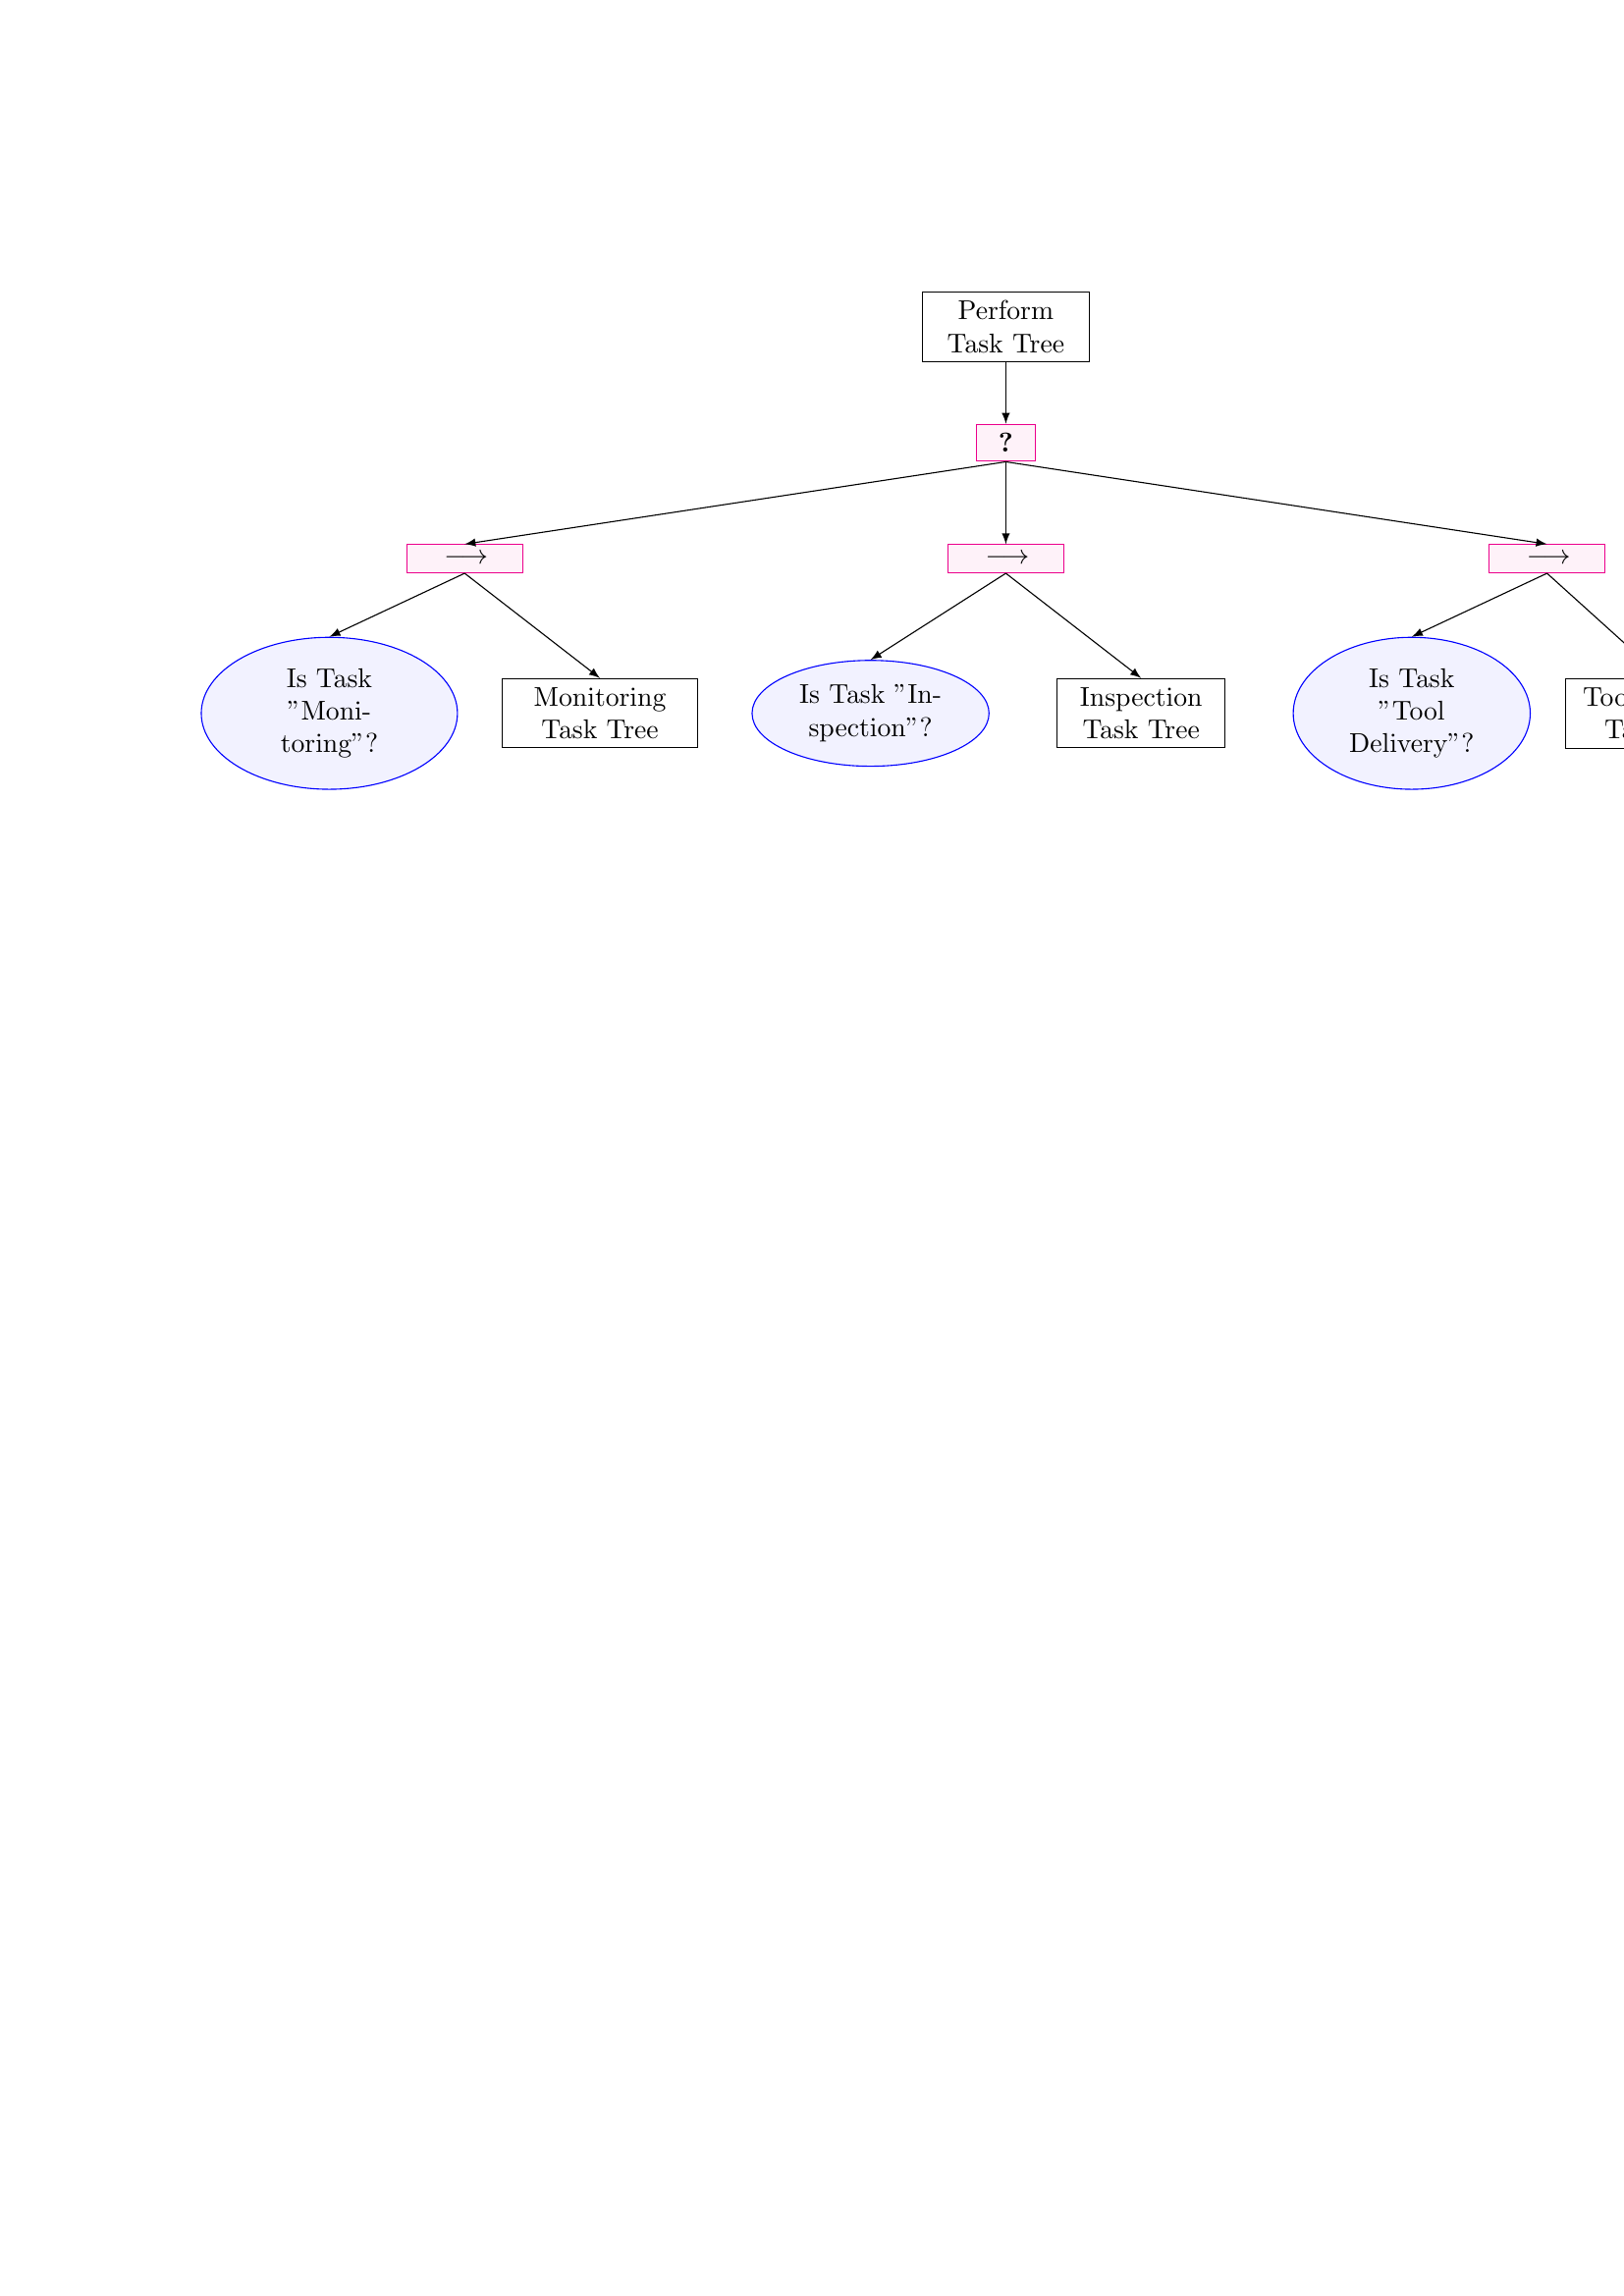
\begin{tikzpicture}
			    \node (PerformTaskTree) at (0,0) [text centered, fill=white, draw, rectangle, minimum width=1.5cm, text width=5.5em]{Perform Task Tree};
        		
        		\node (TaskFallback) at ($(PerformTaskTree) + (0,-1.5)$) [text centered, fill=magenta!5, draw=magenta, rectangle, minimum width=0.5cm, text width=1.5em]{\textbf{?}};
        		\draw[-latex] (PerformTaskTree.south) -- (TaskFallback.north);
        		
        		\node (MonitorSequence) at ($(TaskFallback) + (-7,-1.5)$) [text centered, fill=magenta!5, draw=magenta, rectangle, minimum width=1.5cm, text width=1.5em]{$\longrightarrow$};
        		\draw[-latex] (TaskFallback.south) -- (MonitorSequence.north);
        		\node (InspectSequence) at ($(TaskFallback) + (0,-1.5)$) [text centered, fill=magenta!5, draw=magenta, rectangle, minimum width=1.5cm, text width=1.5em]{$\longrightarrow$};
        		\draw[-latex] (TaskFallback.south) -- (InspectSequence.north);
        		\node (DeliverSequence) at ($(TaskFallback) + (7,-1.5)$) [text centered, fill=magenta!5, draw=magenta, rectangle, minimum width=1.5cm, text width=1.5em]{$\longrightarrow$};
        		\draw[-latex] (TaskFallback.south) -- (DeliverSequence.north);
        		
        		\node (IsTaskMonitor) at ($(MonitorSequence) + (-1.75,-2)$) [text centered, fill=blue!5, draw=blue, ellipse, minimum width=1.5cm, text width=6em]{Is Task "Monitoring"?};
        		\draw[-latex] (MonitorSequence.south) -- (IsTaskMonitor.north);
        		\node (MonitorTree) at ($(MonitorSequence) + (1.75, -2)$) [text centered, fill=white, draw, rectangle, minimum width=1.5cm, text width=6.5em]{Monitoring Task Tree};
        		\draw[-latex] (MonitorSequence.south) -- (MonitorTree.north);
        		\node (IsTaskInspect) at ($(InspectSequence) + (-1.75,-2)$) [text centered, fill=blue!5, draw=blue, ellipse, minimum width=1.5cm, text width=5.5em]{Is Task "Inspection"?};
        		\draw[-latex] (InspectSequence.south) -- (IsTaskInspect.north);
        		\node (InspectTree) at ($(InspectSequence) + (1.75, -2)$) [text centered, fill=white, draw, rectangle, minimum width=1.5cm, text width=5.5em]{Inspection Task Tree};
        		\draw[-latex] (InspectSequence.south) -- (InspectTree.north);
        		\node (IsTaskDeliver) at ($(DeliverSequence) + (-1.75,-2)$) [text centered, fill=blue!5, draw=blue, ellipse, minimum width=1.5cm, text width=5.5em]{Is Task "Tool Delivery"?};
        		\draw[-latex] (DeliverSequence.south) -- (IsTaskDeliver.north);
        		\node (DeliverTree) at ($(DeliverSequence) + (1.5, -2)$) [text centered, fill=white, draw, rectangle, minimum width=1.5cm, text width=6.5em]{Tool Delivery Task Tree};
        		\draw[-latex] (DeliverSequence.south) -- (DeliverTree.north);
        		
		    \end{tikzpicture}}
		\caption{Behaviour Tree: Perform Task Tree}
		\label{fig:PerformTasksTree}
	\end{center}
\end{figure}

The \emph{Perform Task Tree} checks which is the first task in the queue, which is the task that should be executed at that moment. This tree does not require much more explanation, it simply connects the \emph{Main Tree} with the corresponding \emph{Task sub-tree}. At this point, instead of sub-trees, it would be possible to directly place \emph{Leaf} nodes that give control to the appropriate low-level controller, starting to execute the task directly. However, it was decided that the full control would not be given to the low-level controllers until the \gls{ACW} is close enough to the area where the task takes place.

In Figures \ref{fig:MonitorTree}, \ref{fig:InspectTree} and \ref{fig:DeliverToolTree} are depicted the sub-trees that run Safety, Inspection, and Physical tasks, respectively. They all guide the \gls{ACW} close enough to where the low-level controllers need to be called (e.g., close to a worker to monitor or a place to inspect) and then, control is given to the corresponding one. These low-level controllers run on board the corresponding \glspl{ACW} and communicate their results (success or failure) asynchronously back to the \emph{Agent Behaviour Manager}, so that the \gls{BT} can continue running.

In the following, the functioning of each of these sub-trees is described, as well as the details of each of the tasks that have not yet been explained.

\subsection{Inspection task tree}
\label{sec:InspectionTaskTree}
This \gls{BT} is quite simple as the task is just to visit a series of points and stop at each one to take pictures (see Fig. \ref{fig:InspectTree}).

\begin{figure}[ht]
	\begin{center}
		\scalebox{0.9}{
			\begin{tikzpicture}
			    \node (InspectTree) at (0,0) [text centered, fill=white, draw, rectangle, minimum width=1.5cm, text width=5.5em]{Inspection Task Tree};
        		
        		\node (InspectTaskSequence) at ($(InspectTree) + (0,-1.5)$) [text centered, fill=magenta!5, draw=magenta, rectangle, minimum width=1.5cm, text width=1.5em]{$\longrightarrow$};
        		\draw[-latex] (InspectTree.south) -- (InspectTaskSequence.north);
        		
        		\node (NearWPFallback) at ($(InspectTaskSequence) + (-1.5,-1.5)$) [text centered, fill=magenta!5, draw=magenta, rectangle, minimum width=0.5cm, text width=0.5em]{\textbf{?}};
        		\draw[-latex] (InspectTaskSequence.south) -- (NearWPFallback.north);
        		\node (Inspect) at ($(InspectTaskSequence) + (1.5,-1.5)$) [text centered, fill=blue!5, draw=blue, rectangle, minimum width=1.5cm, text width=5.5em]{Inspect};
        		\draw[-latex] (InspectTaskSequence.south) -- (Inspect.north);
        		
        		\node (IsUAVnearWP) at ($(NearWPFallback) + (-1.75,-2)$) [text centered, fill=blue!5, draw=blue, ellipse, minimum width=1.5cm, text width=5.5em]{Is \gls{ACW} near WP?};
        		\draw[-latex] (NearWPFallback.south) -- (IsUAVnearWP.north);
        		\node (GoNearWP) at ($(NearWPFallback) + (1.75, -2)$) [text centered, fill=blue!5, draw=blue, rectangle, minimum width=1.5cm, text width=6.5em]{Go near WP};
        		\draw[-latex] (NearWPFallback.south) -- (GoNearWP.north);
		    \end{tikzpicture}}
		\caption{Behaviour Tree: sub-tree that controls the inspection tasks}
		\label{fig:InspectTree}
	\end{center}
\end{figure}

As mentioned above, control is handed over to the low-level controllers when the \gls{ACW} is close enough to the area where the task takes place. The \emph{Reactive Sequence Control} node behind the root of this sub-tree is in charge of checking this condition at any moment, stopping the low-level controller if it is no longer fulfilled.

All the information that the \gls{BT} needs to operate is known in advance by the \emph{Agent Behaviour Manager}, either because it has received it through one of the interfaces represented in Figure \ref{fig:NodeDiagram}, or because it has calculated it itself in one of the functions that are executed in the main while loop. In particular, to check if the \gls{ACW} is close to the points to be inspected, the information received from the \emph{\gls{ACW}'s autopilot} is used against the points in the list of \glspl{WP} to be inspected. If necessary, the \emph{Action} node \emph{Go near \gls{WP}} is executed, which connects to the low-level controller in charge and gives as target location the nearest \gls{WP} in the list. Once there, the low-level controller that executes this task is called.

\subsection{Monitoring task tree}
\label{sec:MonitoringTaskTree}
As can it be seen in Figure \ref{fig:MonitorTree}, this \gls{BT} follows the same structure as the previous one. The only differences are the \emph{Leaf} nodes.

\begin{figure}[ht]
	\begin{center}
		\scalebox{0.9}{
			\begin{tikzpicture}
			    \node (MonitorTree) at (0,0) [text centered, fill=white, draw, rectangle, minimum width=1.5cm, text width=5.5em]{Monitoring Task Tree};
        		
        		\node (MonitorTaskSequence) at ($(MonitorTree) + (0,-1.5)$) [text centered, fill=magenta!5, draw=magenta, rectangle, minimum width=1.5cm, text width=1.5em]{$\longrightarrow$};
        		\draw[-latex] (MonitorTree.south) -- (MonitorTaskSequence.north);
        		
        		\node (NearHumanFallback) at ($(MonitorTaskSequence) + (-1.5,-1.5)$) [text centered, fill=magenta!5, draw=magenta, rectangle, minimum width=0.5cm, text width=1.5em]{\textbf{?}};
        		\draw[-latex] (MonitorTaskSequence.south) -- (NearHumanFallback.north);
        		\node (MonitorHumanTarget) at ($(MonitorTaskSequence) + (1.5,-1.5)$) [text centered, fill=blue!5, draw=blue, rectangle, minimum width=1.5cm, text width=5.5em]{Monitor};
        		\draw[-latex] (MonitorTaskSequence.south) -- (MonitorHumanTarget.north);
        		
        		\node (IsUAVnearHumanTarget) at ($(NearHumanFallback) + (-2,-2)$) [text centered, fill=blue!5, draw=blue, ellipse, minimum width=1.5cm, text width=6.5em]{Is \gls{ACW} near Human Target?};
        		\draw[-latex] (NearHumanFallback.south) -- (IsUAVnearHumanTarget.north);
        		\node (GoNearHuman) at ($(NearHumanFallback) + (1.55, -2)$) [text centered, fill=blue!5, draw=blue, rectangle, minimum width=1.5cm, text width=6.5em]{Go near Human Target};
        		\draw[-latex] (NearHumanFallback.south) -- (GoNearHuman.north);
		    \end{tikzpicture}}
		\caption{Behaviour Tree: sub-tree that controls the safety monitoring tasks}
		\label{fig:MonitorTree}
	\end{center}
	\vspace{-1em}
\end{figure}

In this case, the position of the operator to be monitored is known from communications with the \emph{Human Tracker} node (see Figure \ref{fig:NodeDiagram}). If the \gls{ACW} is not close enough, the \gls{BT} will call the low-level controller giving it this time the position of the operator as a target. Once the \gls{UAV} is in a position close to the worker, control is passed to the low-level controller in charge of this task. The information needed by this node is the \emph{Monitoring Number}, the \emph{Monitoring Distance}, the \emph{list of \glspl{ACW}' \glspl{ID}}, and the formation to be maintained during the flight, which will be chosen by the \emph{High-Level Planner} from a set of predefined formations based on the monitoring number (see Table \ref{tab:shareddata}). Finally, it is worth mentioning that an \gls{ACW} could be added or removed from the formation at any time by updating the parameters of the task, or even due to availability.

\subsection{Tool delivery task tree}
\label{sec:ToolDeliveryTaskTree}
This tree is a bit more complex, as the task involves several steps (see Fig. \ref{fig:DeliverToolTree}). First, it picks up the requested tool in case the \gls{ACW} does not have it yet. This part involves travelling to the station to pick up the tool in case the \gls{UAV} is not already there. The second part of the task is the process of approaching the operator. After all this, the low-level controller can be activated to carry out the delivery of the tool through a physical interaction between the operator and the \gls{ACW}.

\begin{figure}[ht]
	\begin{center}
		\scalebox{0.85}{
			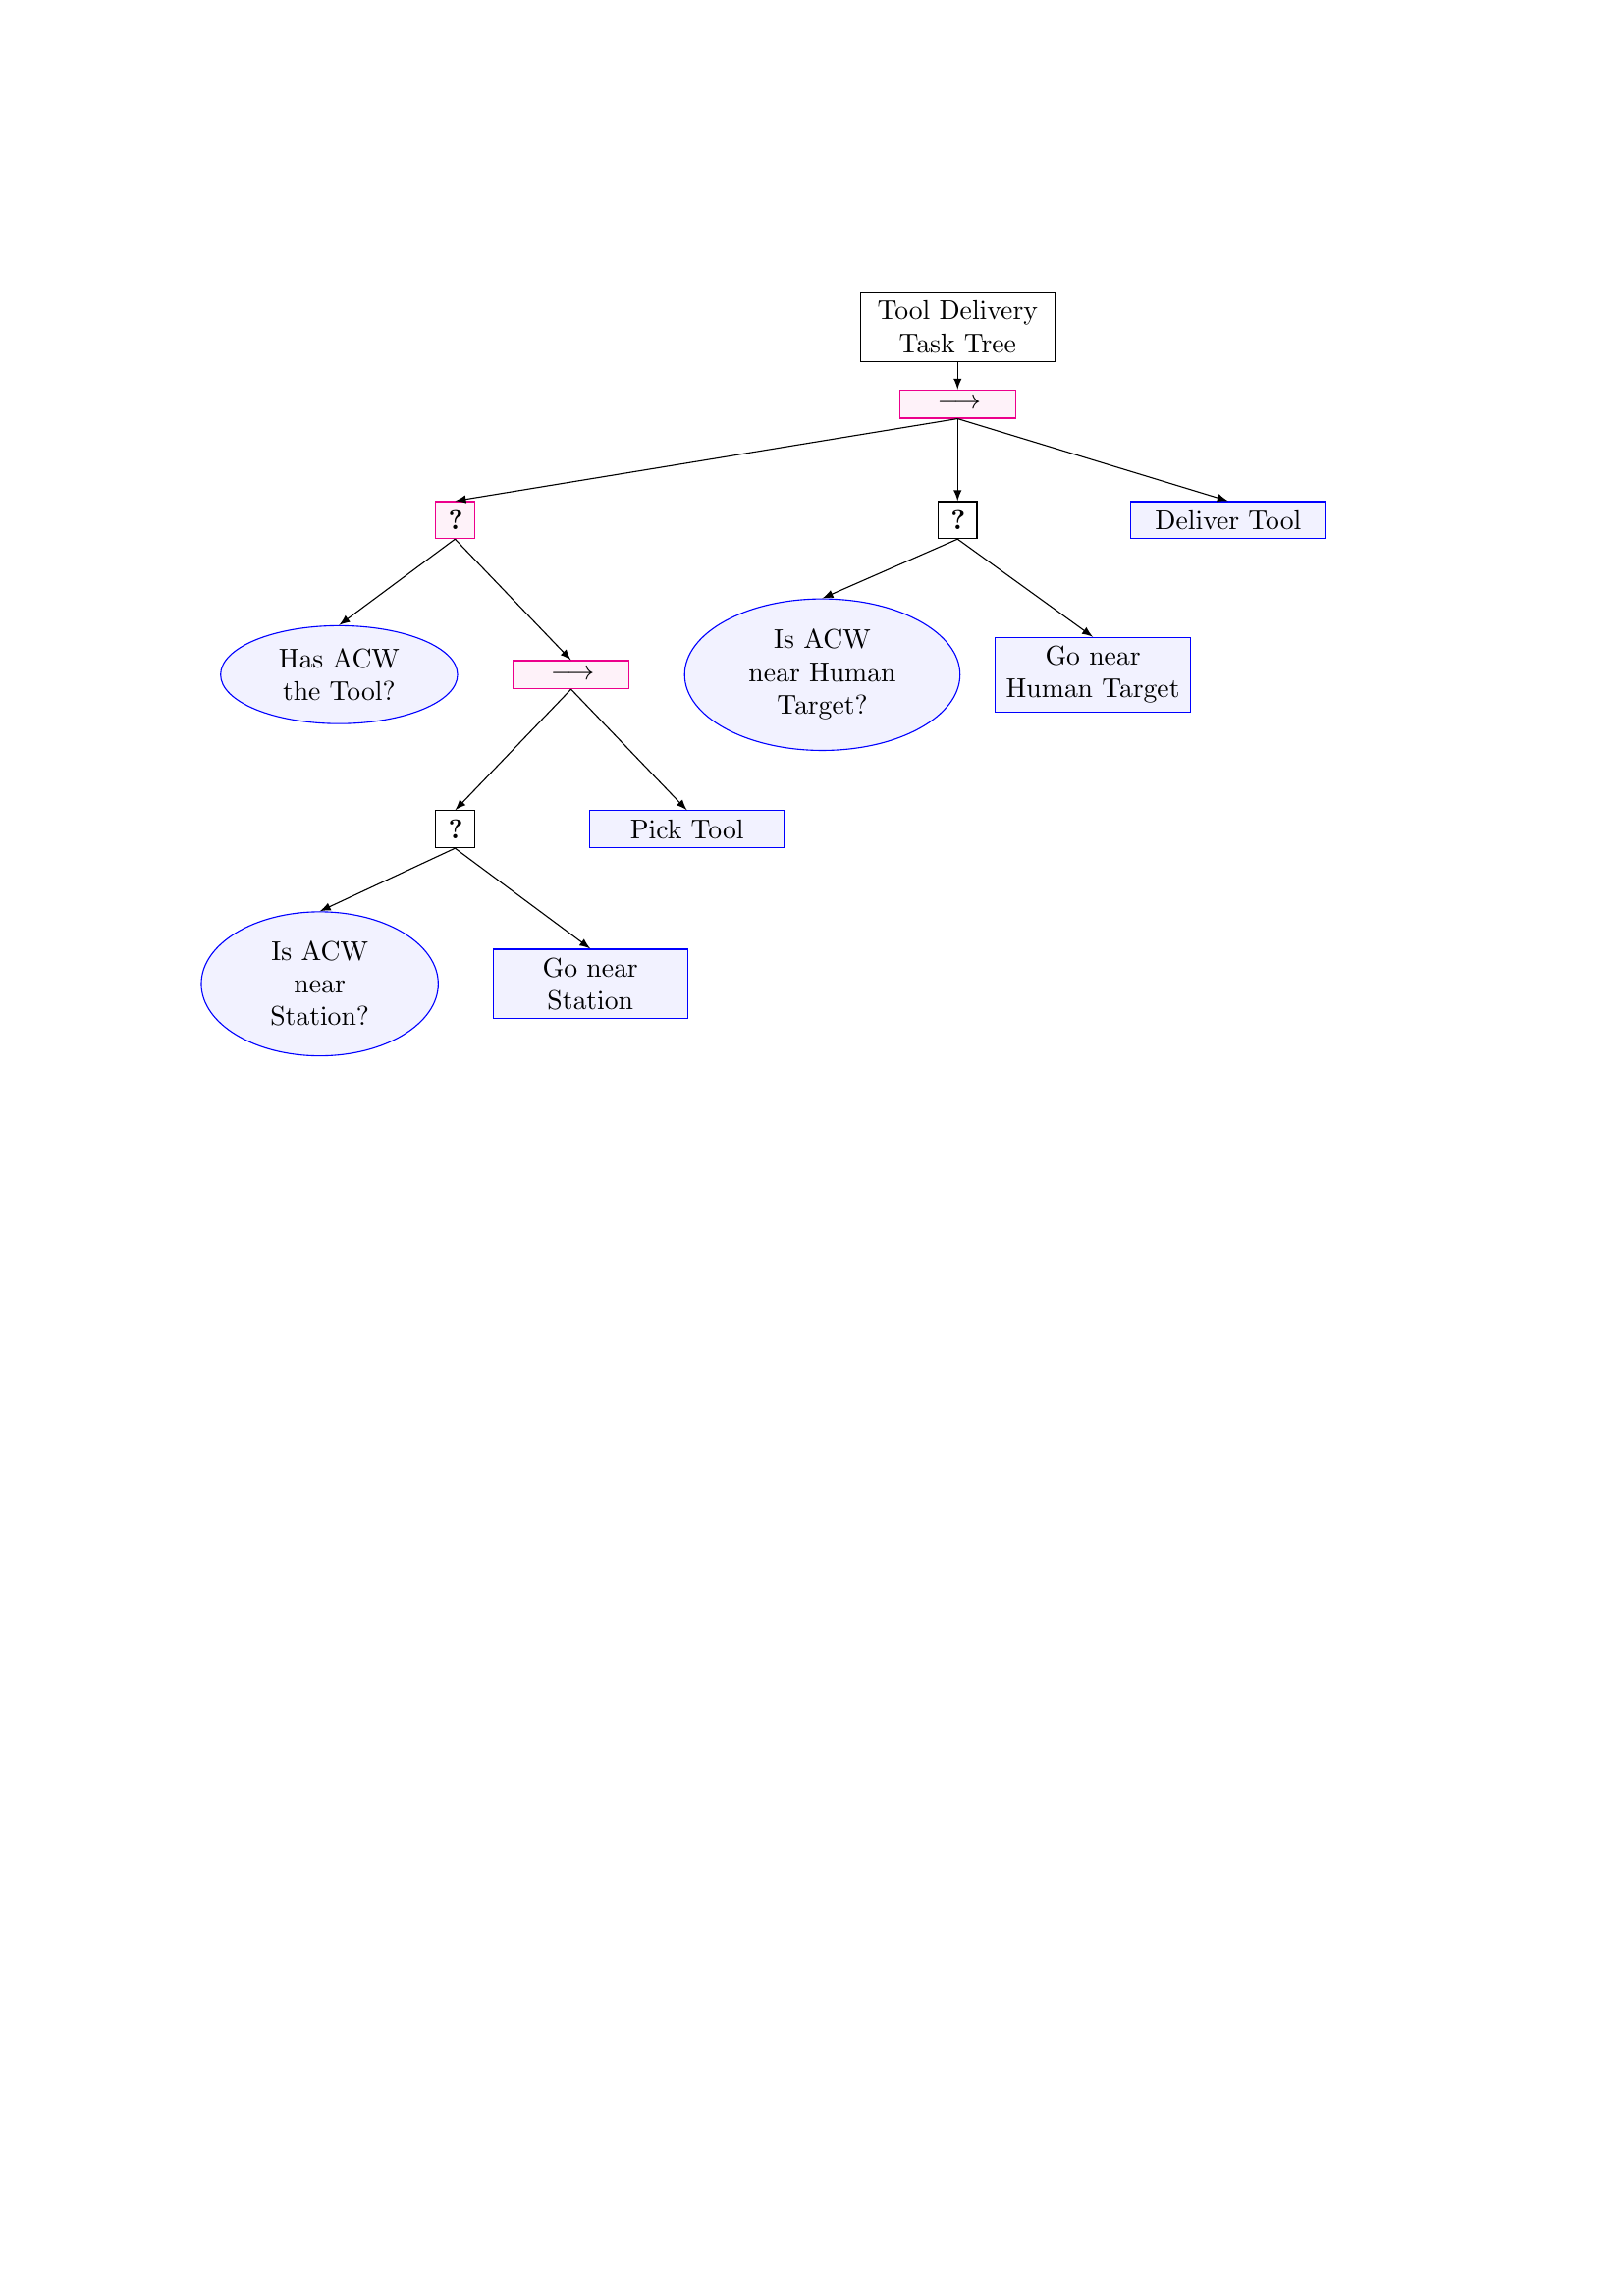
\begin{tikzpicture}
			    \node (DeliverTree) at (0,0) [text centered, fill=white, draw, rectangle, minimum width=1.5cm, text width=6.5em]{Tool Delivery Task Tree};
			    
			    \node (DeliverTaskSequence) at ($(DeliverTree) + (0,-1)$) [text centered, fill=magenta!5, draw=magenta, rectangle, minimum width=1.5cm, text width=1.5em]{$\longrightarrow$};
        		\draw[-latex] (DeliverTree.south) -- (DeliverTaskSequence.north);

				\node (ToolFallback) at ($(DeliverTaskSequence) + (-6.5,-1.5)$) [text centered, fill=magenta!5, draw=magenta, rectangle, minimum width=0.5cm, text width=0.5em]{\textbf{?}};
        		\draw[-latex] (DeliverTaskSequence.south) -- (ToolFallback.north);
        		\node (HumanFallback) at ($(DeliverTaskSequence) + (0,-1.5)$) [text centered, fill=white, draw, rectangle, minimum width=0.5cm, text width=0.5em]{\textbf{?}};
        		\draw[-latex] (DeliverTaskSequence.south) -- (HumanFallback.north);
        		%\node (PermissionFallback) at ($(DeliverTaskSequence) + (6.5,-1.5)$) [text centered, fill=magenta!5, draw=magenta, rectangle, minimum width=0.5cm, text width=0.5em]{\textbf{?}};
        		%\draw[-latex] (DeliverTaskSequence.south) -- (PermissionFallback.north);
				\node (DeliverTool) at ($(DeliverTaskSequence) + (3.5,-1.5)$) [text centered, fill=blue!5, draw=blue, rectangle, minimum width=1.5cm, text width=6.5em]{Deliver Tool};
        		\draw[-latex] (DeliverTaskSequence.south) -- (DeliverTool.north);

				\node (hasACWtheTool) at ($(ToolFallback) + (-1.5,-2)$) [text centered, fill=blue!5, draw=blue, ellipse, minimum width=1.5cm, text width=5.5em]{Has \gls{ACW} the Tool?};
        		\draw[-latex] (ToolFallback.south) -- (hasACWtheTool.north);
        		\node (PickToolSequence) at ($(ToolFallback) + (1.5,-2)$) [text centered, fill=magenta!5, draw=magenta, rectangle, minimum width=1.5cm, text width=1.5em]{$\longrightarrow$};
        		\draw[-latex] (ToolFallback.south) -- (PickToolSequence.north);
        		\node (IsUAVnearHuman) at ($(HumanFallback) + (-1.75,-2)$) [text centered, fill=blue!5, draw=blue, ellipse, minimum width=1.5cm, text width=6.5em]{Is \gls{ACW} near Human Target?};
        		\draw[-latex] (HumanFallback.south) -- (IsUAVnearHuman.north);
        		\node (GoNearHuman) at ($(HumanFallback) + (1.75, -2)$) [text centered, fill=blue!5, draw=blue, rectangle, minimum width=1.5cm, text width=6.5em]{Go near Human Target};
        		\draw[-latex] (HumanFallback.south) -- (GoNearHuman.north);
        		%\node (DeliverSequence) at ($(PermissionFallback) + (-2.25,-2)$) [text centered, fill=white, draw, rectangle, minimum width=1.5cm, text width=1.5em]{$\longrightarrow$};
        		%\draw[-latex] (PermissionFallback.south) -- (DeliverSequence.north);
        		%\node (ForceFailure) at ($(PermissionFallback) + (2.25, -2)$) [text centered, fill=orange!5, draw=orange, rectangle, minimum width=1.5cm, text width=5.5em]{Force Failure};
        		%\draw[-latex] (PermissionFallback.south) -- (ForceFailure.north);


        		\node (StationFallback) at ($(PickToolSequence) + (-1.5,-2)$) [text centered, fill=white, draw, rectangle, minimum width=0.5cm, text width=0.5em]{\textbf{?}};
        		\draw[-latex] (PickToolSequence.south) -- (StationFallback.north);
        		\node (PickTool) at ($(PickToolSequence) + (1.5, -2)$) [text centered, fill=blue!5, draw=blue, rectangle, minimum width=1.5cm, text width=6.5em]{Pick Tool};
        		\draw[-latex] (PickToolSequence.south) -- (PickTool.north);
        		%\node (hasUAVpermission) at ($(DeliverSequence) + (-3.25,-2)$) [text centered, fill=white, draw, ellipse, minimum width=1.5cm, text width=5.5em]{Has  permission?};
        		%\draw[-latex] (DeliverSequence.south) -- (hasUAVpermission.north);
        		%\node (DeliverTool) at ($(DeliverSequence) + (0, -2)$) [text centered, fill=white, draw, rectangle, minimum width=1.5cm, text width=6.5em]{Tool Delivery};
        		%\draw[-latex] (DeliverSequence.south) -- (DeliverTool.north);
        		%\node (Retreat) at ($(DeliverSequence) + (3, -2)$) [text centered, fill=white, draw, rectangle, minimum width=1.5cm, text width=4.5em]{Retreat};
        		%\draw[-latex] (DeliverSequence.south) -- (Retreat.north);
        		%\node (WaitFallback) at ($(ForceFailure) + (0,-2)$) [text centered, fill=magenta!5, draw=magenta, rectangle, minimum width=0.5cm, text width=0.5em]{\textbf{?}};
        		%\draw[-latex] (ForceFailure.south) -- (WaitFallback.north);
        		
        		\node (IsUAVnearStation) at ($(StationFallback) + (-1.75,-2)$) [text centered, fill=blue!5, draw=blue, ellipse, minimum width=1.5cm, text width=5.5em]{Is \gls{ACW} near Station?};
        		\draw[-latex] (StationFallback.south) -- (IsUAVnearStation.north);
        		\node (GoNearStation) at ($(StationFallback) + (1.75, -2)$) [text centered, fill=blue!5, draw=blue, rectangle, minimum width=1.5cm, text width=6.5em]{Go near Station};
        		\draw[-latex] (StationFallback.south) -- (GoNearStation.north);
        		%\node (TimeoutSequence) at ($(WaitFallback) + (-1.5,-2)$) [text centered, fill=white, draw, rectangle, minimum width=1.5cm, text width=1.5em]{$\longrightarrow$};
        		%\draw[-latex] (WaitFallback.south) -- (TimeoutSequence.north);
        		%\node (Wait) at ($(WaitFallback) + (1.5, -2)$) [text centered, fill=white, draw, rectangle, minimum width=1.5cm, text width=6.5em]{Wait for Permission};
        		%\draw[-latex] (WaitFallback.south) -- (Wait.north);

        		%\node (Timeout) at ($(TimeoutSequence) + (-3.25,-2)$) [text centered, fill=white, draw, ellipse, minimum width=1.5cm, text width=5.5em]{Timeout?};
        		%\draw[-latex] (TimeoutSequence.south) -- (Timeout.north);
        		%\node (GoNearStation) at ($(TimeoutSequence) + (0, -2)$) [text centered, fill=white, draw, rectangle, minimum width=1.5cm, text width=6.5em]{Go near Station};
        		%\draw[-latex] (TimeoutSequence.south) -- (GoNearStation.north);
        		%\node (DropTool) at ($(TimeoutSequence) + (3.25, -2)$) [text centered, fill=white, draw, rectangle, minimum width=1.5cm, text width=6.5em]{Drop the Tool};
        		%\draw[-latex] (TimeoutSequence.south) -- (DropTool.north);
		    \end{tikzpicture}}
		\caption{Behaviour Tree: sub-tree that controls the tool delivery tasks}
		\label{fig:DeliverToolTree}
	\end{center}
\end{figure}

Again, the location of the operator and the position of the \gls{ACW} is provided by the \emph{\gls{ACW}'s autopilot} and \emph{Human Tracker} blocks. The position of the fixed elements, in this case, the station where the tools are placed, is available among the information read by the \emph{Agent Behaviour Manager} node from the configuration file during its initialisation.

In this case, the low-level controller that delivers the tool will be in charge of requesting the operator's permission to approach. In the meantime, it will have to wait. When it gets the permission, it is time to make the delivery. If too much time elapses without the operator giving the order, the task will be aborted and the tool will be returned to the station.

\section{High- and low-level blocks faking}
\label{sec:faking}
The work in this thesis consisted of programming one of the software layers that make up a software architecture. As there are still parts of the software architecture that are not yet available for integration, temporary solutions have had to be programmed to simulate their action during testing. This section will discuss those parts of the code whose mission is to fool both \emph{High-Level Planner} and \emph{Agent Behaviour Manager} blocks into believing that they are communicating with the real blocks, or to provide functions necessary for the execution to progress.

Low-level controllers have been faked in different ways. For \gls{BT}'s \emph{Action} nodes of the \emph{"Go To"} type, the \emph{GoToWaypoint} \gls{ROS} service available in the \gls{UAL} tool is called instead, which leads the \gls{UAV} to the entered coordinates (although it does not take obstacles into account). For more complex \emph{Action} nodes such as \emph{Inspect}, \emph{Monitor}, \emph{Deliver Tool} or \emph{Pick Tool}, a function is simply called which sleeps the \emph{Action} node for a while simulating that the low-level controller has been called and is waiting for a response. For these \emph{Action} nodes, the response of the \emph{tick} function will be \emph{RUNNING} while sleeping, and either \emph{FAILURE} or \emph{SUCCESS} depending on whether their execution is halted or not. During sleeping time the rest of the tree continues running. The \emph{Recharge} node also calls some low-level controllers. In this particular case it was decided to ignore the call and simply land the \gls{UAV} on the charging station.

On the other hand, since \gls{UAL} does not allow battery control, and the battery level that is available for reading remains static throughout the simulation, it has been necessary to create a block that simulates the evolution of the battery both during flight and during recharging. This block is programmed in such a way that at initialisation it reads the configuration file, thus having the position of the charging stations, and also subscribes to the information published by the \emph{\gls{ACW}'s autopilot} to which it is faking the battery in order to know its position and status. If the \gls{UAV} is in the air, the battery will be periodically decremented. Otherwise, the battery will remain static unless the \gls{UAV} is over a charging station, in which case the battery will periodically increment. The battery percentage and charge/discharge rate is externally configurable at any time during the simulation. In addition, for ease of testing, this block allows for different modes of operation that can among other things make the battery static. The false battery level is periodically published in a similar direction to the one used for the real battery.

Finally, as mentioned in the section \ref{sec:Centralised module:TaskPlanner}, the algorithm in charge of performing the distribution of \glspl{WP} for an inspection task among the different selected \glspl{ACW} has been forged. Normally, this algorithm is executed inside the low-level controller itself which is called by the \emph{Inspect Action} node which can be found in the tree of the figure \ref{fig:InspectTree}. However, as this \emph{Action} node has been completely forged, a distribution of \glspl{WP} has been made within the task planning algorithm. It simply assigns, in order, one \gls{WP} from the list to each selected \gls{ACW} until the list of \glspl{WP} is exhausted.
%
%\chapter{Results}
\label{ch:Results}

\lettrine[lraise=-0.1, lines=2, loversize=0.2]{L}{o}rem itsum

\section{Task planning}
\label{sec:TaskPlanning}

\subsection{Battery}
\label{subsec:Battery}

\subsection{Connection lost}
\label{subsec:ConnectionLost}

\subsection{Replanning}
\label{subsec:Replanning}


\section{Drone behaviour manager results}
\label{sec:DroneBehavioutManagerResults}

\subsection{Battery management}
\label{subsec:BatteryManagement}

\subsection{Connection lost management}
\label{subsec:ConnectionLostManagement}

\subsection{Replanning management}
\label{subsec:ReplanningManagement}


\section{Simulations}
\label{sec:Simulations}

\subsection{One drone simulations}
\label{subsec:OneDroneSimulations}

\subsection{Multi-drone simulations}
\label{subsec:Multi-droneSimulations}


%
% \chapter{Conclusions and future work}
\label{ch:ConclusionsAndFutureWork}

\section{Conclusions}
\label{sec:Conclusions}
%% Comentar los objetivos marcados:
In this work, a task planning approach has been developed with the capability to perform mission planning for multi-\gls{UAV} teams. The system has sufficient cognitive capability to control multiple \glspl{UAV} operating as co-workers in dynamic environments safely. Simulations have demonstrated the system's ability to detect emergency situations and act in a safe way by executing contingency plans autonomously while calculating a new plan to follow that takes into account the unforeseen events that have occurred. The design of the system proposed two blocks: a centralised block on the ground in charge of optimal mission planning; and distributed blocks on board each of the \glspl{ACW} to allow the system to be robust to failures and have enough cognitive capacity to react to unforeseen events by recalculating the optimal plan. In this way, an efficient execution of tasks and a better use of resources is achieved, which translates into greater combined autonomy for the \gls{UAV} team.

The system has been designed in \gls{ROS} and the communications between the different software layers and the different blocks of each layer have been carried out using the tools offered by \gls{ROS}. This facilitates the integration of the system developed in other robotics projects that require a task planning system with these or similar characteristics. The use of \glspl{BT} for the design of the \gls{UAV} behaviour manager has great advantages over conventional \glspl{FSM}. This technique makes it possible to generate complex behaviours with numerous states without having to worry about taking into account each of the transitions between these states, as happens with \glspl{FSM}, in which the number of transitions grows exponentially with the number of states. The characteristics of the library used to program this part of the system make it easy to maintain, modify or extend. Moreover, thanks to its modular nature, this block can be reused in parts or in its entirety in any other project. The designed \gls{BT}, although it can be improved, has demonstrated in the simulations that works fairly well, laying the foundations for programming more complex behaviours in the future and serving as an example for the aerial robotics community, which can use it as a starting point for other applications. 

With respect to the block in charge of mission planning, the \emph{High-Level Planner}, it has so far demonstrated the ability to generate coherent plans in the conditions in which it has been tested and has also shown itself capable of recalculating these plans online in reaction to unforeseen events of different natures. The achieved solution is able to plan the mission taking into account imposed constraints such as the type of each \gls{ACW}, the priority of each of the tasks and the battery level of each of the \glspl{UAV}, being able to calculate plans for missions consisting of an indefinite number of tasks and \glspl{ACW}. Regarding the optimality of the plans generated by this block, it should be noticed that it has not been implemented any solution to approximate the optimal plan, but a heuristic solution based on a cost function that is calculated for each of the \glspl{ACW} with each of the tasks. However, this type of solution should be enough for initial tests in the targeted scenarios, are composed of few tasks and \glspl{ACW}. The solution reached, in this context, is a valid approximation towards a planning algorithm that generates a close-to-optimal plan.

\section{Future work}
\label{sec:FutureWork}
As part of the future work, the techniques developed in this work will be validated in a real environment with real \glspl{UAV}. In addition, the system will be used as a starting point for a PhD thesis in which it will be attempted to refine and improve the design of the \emph{Agent Behaviour Manager} block, as well as to develop a planning algorithm that generates a real approximation to the optimal plan for each situation. To this end, probabilistic decision-making algorithms will be introduced into the system, as well as the capacity to learn in real time some characteristics such as the \glspl{UAV}' battery consumption or human's intentions, thus anticipating unforeseen events and applying contingency plans. This would provide a greater robustness against failures and highly dynamic environments.

A first improvement for the planner with respect to the current version could be the incorporation of \emph{reload} tasks that, instead of being requested by human operators like the rest of the tasks, would be incorporated by the \emph{High-Level Planner} into the task queue, thus separating emergency reloads (or reloads that are executed when an agent is idle) from reloads carried out as part of the plan. Implementing this change in the \gls{BT} would mean modifying the \emph{Perform Task} tree to contemplate this new task in the design of the tree, a change that could be carried out by reusing and slightly adapting the trees used for the \emph{Inspection} and \emph{Safety Monitoring} tasks, taking advantage of the reusability of the \glspl{BT}.

In addition, in future work, it is intended to investigate the use of mixed reality technologies also for inspection applications with multi-\gls{UAV} teams, combining views taken from different points to recreate more complete visual environments for the operator, and improving the human-machine interaction of the system during collaborative tasks.

\endinput

\chapter{Conclusiones and trabajo futuro}
\label{ch:ConclusionsAndFutureWork}
\section{Conclusiones}
\label{sec:Conclusions}
En este trabajo se ha desarrolado un planificador de tareas con capacidad para realizar la planificación de misiones para equipos multi-UAV. El sistema tiene la capacidad cognitiva suficiente para controlar a múltiples UAVs que funcionen como co-trabajadores en entornos dinámicos de forma segura. Las simulaciones realizadas han demostrado la capacidad que tiene el sistema para detectar situaciones de emergencia y actuar de forma segura ejecutando planes de contingencia de forma autónoma mientras se calcula un nuevo plan a seguir que tenga en cuenta los imprevistos que hayan acontecido. El diseño del sistema dividido en un bloque centralizado en tierra encargado de realizar la planificación óptima de la misión y de bloques distribuidos a bordo de cada uno de los ACWs permite que el sistema presente robustez ante fallos y capacidad cognitiva suficiente para reaccionar ante eventos imprevistos recalculando el plan óptimo. De esta forma, se consigue una ejecución eficiente de las tareas y un mejor aprovechamiento de los recursos, que se traduce en una mayor autonomía conjunta del equipo de UAVs.

El sistema se ha diseñado en ROS y las comunicacioens entre las diferentes capas de software y los diferentes bloques de cada capa se han realizado empleando las herramientas que este ofrece. Esto facilita la integración del sistema desarrollado en otros proyectos de robótica que necesiten de un planificador de tareas con estas características o similares. El uso de BT para el diseño del UAV behaviour manager presenta grandes ventajas frente a las FSM convencionales. Esta técnica permite generar comportamientos complejos con numerosos estados sin que haya que preocuparse por tener en cuenta cada una de las transiciones entre esos estados como pasa con las FSM, en las que el número de transiciones crece exponencialmente con el número de estados. Las características de la librería empleada para programar esta parte del sistema hacen que sea facil de mantener, de modificar o de amplicar. Además, gracias a su caracter modular, este bloque puede ser reutilizado tanto a partes como en su totalidad en cualquier otro proyecto. El BT diseñado, aunque mejorable, ha demostrado en las simulaciones realizadas que funciona bastante bien, sentando las bases para programar comportamientos más complejos en el futuro y sirviendo de ejemplo para la comunidad de robótica aérea, que podrá emplearlo como punto de partida para otras aplicaciones. 

Respecto al bloque que se encarga de la planificación de la misión, el High-Level Planner, decir que hasta el momento ha demostrado tener la capacidad para general planes con sentido en las condiciones en las que se le ha puesto a prueba y que además ha demostrado ser capaz de recalcular dichos planes en línea como reacción a eventos imprevistos de diferente naturaleza. La solición alcanzada es capaz de planificar la misión teniento en cuenta resticciones impuestas como el tipo de cada ACW, la prioridad de cada una de las tareas y el nivel de autonomía de cada uno de los UAVs, siendo capaz de calcular planes para misiones formadas por una cantidad indefinida de tareas y ACWs. Respecto a la optimalidad de los planes generados por este bloque hay que decir que no se ha implementado ningún algoritmo que realice una búsqueda o aproximación del plan óptimo, sino que se ha diseñado una solución basada en una funcion de costes que se calcula para cada uno de los ACWs con cada una de las tareas. Sin embargo, este trabajo forma parte de un proyecto que tendrá aplicaciones reales en unas condiciones definidas. Por tanto, está justificado alejarse de análisis académicos en los que se busca aproximar el plan óptimo en misiones con un número indeterminado de tareas y de ACWs y analizar en su lugar al planificador en escenarios compuestos por pocas tareas y ACWs. La solución alcanzada, en este contexto, es una aproximación válida hacia un algoritmo de planificación que genere un plan próximo al óptimo.

\section{Trabajo futuro}
\label{sec:FutureWork}
Como parte del trabajo futuro se realizará una validación en un entorno real con equivos reales de las técnicas desarrolladas en este trabajo. Además, el sistema desarrollado en este trabajo se empleará como punto de partida de una tesis doctoral en la que se tratará de pulir y mejorar el diseño del Agent Behaviour Manager, así como de desarrollar un algoritmo de planificación que genere una aproximación real al plan óptimo de cada situación. Para ello se introducirán al sistema algoritmos heurísticos aleatorios, así como la capacidad para aprender en tiempo real características como el consumo de la batería de los UAVs, anticipándose de esta forma a eventos imprevistos aplicando planes de contingencia, consiguiendo así una mayor robustez ante fallos y extendiendo la autonomía del sistema aún más.

Una primera mejora para el planificador respecto a la versión actual podría ser la incorporación de tareas de tipo Recarga que, en vez de ser solicitadas por operarios humanos como el resto de las tareas, serían incorporadas por el High-Level Planner a la cola de tareas, separando de esta forma las recargas de emergencia o las recargas que se ejecutan cuando un agente se encuentra ocioso, de las recargas llevadas a cabo como parte del plan. Implementar este cambio en el BT supondría modificar el Perform Task Tree para contemplar esta nueva tarea en el diseño del árbol, cambio que se podría llevar a cabo reutilizando y adaptando ligeramente los árboles empleados para las tareas de Inspection y Safety Monitoring aprovechando la reusabilidad de los BTs.

Además, durante la futura tésis, se pretende investigar el uso de tacnologías de realidad mixta también para aplicaciones de inspección con equipos multi-UAV, combinando vistas tomadas desde distintos puntos para recrear entornos visuales más completos para el operario, y mejorando la interacción hombre-máquina del sistema durante tareas colaborativas.

%\endinput

%\chapter{References}
\label{ch:References}



\endinput

%

%%%%%%%%%%%%%%%%%%%%%%%%%%%%%%%%%%%%%%%%%%%%%%%%%%%%%%%%%%%%%%%%%%%%%%%%%%%%%%%
%%%%%%%%%%%%%%%%%%%%%%%%%%%%%%%%%%%%%%%%%%%%%%%%%%%%%%%%%%%%%%%%%%%%%%%%%%%%%%%
%%%%%%% Esto aún no lo he investigado, tengo que ver como va
%%%%%%%%%%%%%%%%%%%%%%%%%%%%%%%%%%%%%%%%%%%%%%%%%%%%%%%%%%%%%%%%%%%%%%%%%%%%%%%
%%%%%%%%%%%%%%%%%%%%%%%%%%%%%%%%%%%%%%%%%%%%%%%%%%%%%%%%%%%%%%%%%%%%%%%%%%%%%%%
%%%%%%% Apéndices
%%:Empezamos con los apéndices, que irían en uno o más ficheros. Es necesario incluir estos ficheros entre el entorno \begin{appendices}....\end{appendices} debido a que se ha deseado utilizar un formato diferente para el título de los apéndices, incluyendo la palabra apéndice, para la numeración de los apéndices, alfabético, y para las cabeceras de las páginas.
%
% \begin{appendices}
%
% \include{apendices/apendices} 
%
% \end{appendices}

%%%%%%%%%%%%%%%%%%%%%%%%%%%%%%%%%%%%%%
%%%%%%%%%%%%%%%%%%%%%%%%%%%%%%%%%%%%%%
%:Empieza todo lo que no constituye el cuerpo en si del libro. Todo lo que va detrás
\backmatter

%:Indice de figuras, coméntese las siguientes líneas si no se desea
\cleardoublepage
\phantomsection

%:Para añadir una línea en blanco en el TOC y separar esta lista
\addtocontents{toc}{\protect\mbox{}\protect\hspace*{0pt}\par}
\addcontentsline{toc}{listasb}{\listfigurename}
\pagestyle{especial}
\listoffigures

%:Indice de tablas, coméntese las siguientes líneas si no se desea
\cleardoublepage
\phantomsection
\addcontentsline{toc}{listasb}{\listtablename}
\pagestyle{especial}
\listoftables

%:Indice de Programas
\cleardoublepage
\phantomsection
\addcontentsline{toc}{listasb}{\lstlistlistingname}
\pagestyle{especial}
\lstlistoflistings

%%%%%%%%%%%%%%%%%%%%%%%%%%%%%%%%%%%%%%%%%%%%%%%%%%%%%%%%%%%%%%%%%%%%%%%%%%%%%%%
%:Bibliografía con biblatex
\nocite{*}
\cleardoublepage
\phantomsection
\addcontentsline{toc}{listasb}{\bibname}
\pagestyle{especial}

\bibliographystyle{IEEEtran}
%\bibliographystyle{amsplain} %flexbib amsplain alpha

%:Fichero con la bibliografía, BIBTEX
\bibliography{bibliography}

% Este fichero .bib se puede generar usando algún gestor de bibliografías. Se recomiendan dos:
% - Zotero
% - Mendeley (con licencia de la US)

%:Índice alfabético de palabras
%\cleardoublepage
%\phantomsection
%\addcontentsline{toc}{listasb}{\indexname}
%\chaptermark{\indexname}
%\printindex


%:Acrónimos
\cleardoublepage
\phantomsection
\addcontentsline{toc}{listasb}{\glossaryname}
\chaptermark{\glossaryname}
\printglossaries


\end{document}
